

\documentclass[a4paper]{article}

\usepackage[english]{babel}
\usepackage{amsmath}
\usepackage{tikz}
\usepackage{listings}
\usepackage{pxfonts}
\usepackage[margin=1in]{geometry}
\usepackage[nottoc]{tocbibind}
\usepackage{xcolor}
\usepackage{float}

\setcounter{MaxMatrixCols}{12}
\usetikzlibrary{arrows.meta,calc}
\tikzset{>={Latex[width=1.2mm,length=2.5mm]}}
\lstset{
	belowcaptionskip=1\baselineskip,
	breaklines=true,
	xleftmargin=\parindent,
	language=C++,
	showstringspaces=false,
	basicstyle=\ttfamily\small,
	keywordstyle=\bfseries\color{green!40!black},
	commentstyle=\itshape\color{purple!40!black},
	identifierstyle=\color{blue},
	stringstyle=\color{orange},
	tabsize=2,
}


\title{THIS WORK IS STILL UNDER DEVELOPMENT Conjugate Gradients Method by Example in Qt/C++}
\author{Krzysztof Napiontek\protect\\knapiontek@gmail.com}
\date{Version 1.0\protect\\\today}

\begin{document}

\maketitle

\begin{abstract}

Work under active development.

\end{abstract}

\tableofcontents

\section{Introduction}

Practical implementation of CGM.

\section{The Realistic Example}

\begin{figure}[H]
\centering
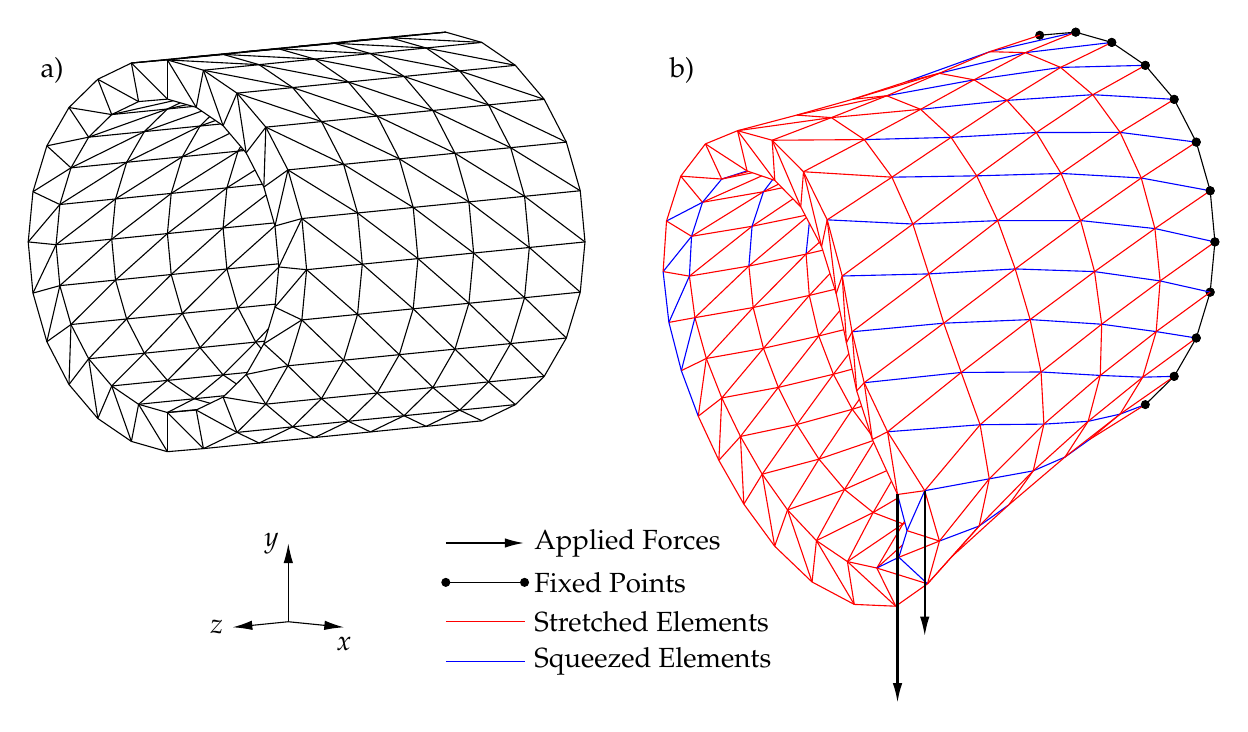
\begin{tikzpicture}
\draw[->] (-6,-2) -- (-5.29289,-2.07059);
\node[below] at (-5.29289,-2.07059) {$x$};
\draw[->] (-6,-2) -- (-6,-1.005);
\node[left] at (-6,-1.005) {$y$};
\draw[->] (-6,-2) -- (-6.70711,-2.07059);
\node[left] at (-6.70711,-2.07059) {$z$};
\draw (-2.23223,2.82352) -- (-2.99958,3.40275);
\draw (-2.23223,2.82352) -- (-2.93934,2.75292);
\draw (-2.23223,2.82352) -- (-2.29247,2.18572);
\draw (-2.56764,2.427) -- (-2.56764,2.427);
\draw (-2.23223,2.82352) -- (-2.29247,3.47335);
\draw (-2.29247,3.47335) -- (-3.17618,4.02032);
\draw (-2.29247,3.47335) -- (-2.99958,3.40275);
\draw (-2.29247,3.47335) -- (-2.46907,4.09092);
\draw (-2.46907,4.09092) -- (-3.4571,4.56355);
\draw (-3.03134,3.93068) -- (-3.03134,3.93068);
\draw (-2.46907,4.09092) -- (-3.17618,4.02032);
\draw (-2.46907,4.09092) -- (-2.75,4.63415);
\draw (-2.75,4.63415) -- (-3.82322,4.99541);
\draw (-2.75,4.63415) -- (-3.4571,4.56355);
\draw (-2.75,4.63415) -- (-3.11612,5.066);
\draw (-3.11612,5.066) -- (-4.24957,5.28648);
\draw (-3.11612,5.066) -- (-3.82322,4.99541);
\draw (-3.11612,5.066) -- (-3.54247,5.35707);
\draw (-3.54247,5.35707) -- (-4.70711,5.41692);
\draw (-3.54247,5.35707) -- (-4.24957,5.28648);
\draw (-3.54247,5.35707) -- (-4,5.48751);
\draw (-4,5.48751) -- (-5.16464,5.37783);
\draw (-4.12509,5.38701) -- (-4.12509,5.38701);
\draw (-4,5.48751) -- (-4.70711,5.41692);
\draw (-4,5.48751) -- (-4.45753,5.44842);
\draw (-4.46244,5.44396) -- (-4.46244,5.44396);
\draw (-4.45753,5.44842) -- (-5.16464,5.37783);
\draw (-4.46782,5.44345) -- (-4.46782,5.44345);
\draw (-3.54247,0.551577) -- (-3.82322,0.686922);
\draw (-3.80403,0.688838) -- (-3.80403,0.688838);
\draw (-3.54247,0.551577) -- (-4.24957,0.480984);
\draw (-3.54247,0.551577) -- (-3.11612,0.757515);
\draw (-3.11612,0.757515) -- (-3.4571,1.04568);
\draw (-3.11612,0.757515) -- (-3.82322,0.686922);
\draw (-3.11612,0.757515) -- (-2.75,1.11627);
\draw (-3.07536,1.54288) -- (-3.07536,1.54288);
\draw (-2.75,1.11627) -- (-3.17618,1.53281);
\draw (-3.31261,1.29624) -- (-3.31261,1.29624);
\draw (-2.75,1.11627) -- (-3.4571,1.04568);
\draw (-2.75,1.11627) -- (-2.46907,1.60341);
\draw (-2.46907,1.60341) -- (-2.99958,2.11512);
\draw (-2.46907,1.60341) -- (-3.17618,1.53281);
\draw (-2.46907,1.60341) -- (-2.29247,2.18572);
\draw (-2.29247,2.18572) -- (-2.93934,2.75292);
\draw (-2.98714,2.24684) -- (-2.98714,2.24684);
\draw (-2.29247,2.18572) -- (-2.99958,2.11512);
\draw (-2.93934,2.75292) -- (-3.70669,3.33216);
\draw (-2.93934,2.75292) -- (-3.64645,2.68233);
\draw (-2.93934,2.75292) -- (-2.99958,2.11512);
\draw (-2.93934,2.75292) -- (-2.99958,3.40275);
\draw (-2.99958,3.40275) -- (-3.88328,3.94973);
\draw (-2.99958,3.40275) -- (-3.70669,3.33216);
\draw (-2.99958,3.40275) -- (-3.17618,4.02032);
\draw (-3.17618,4.02032) -- (-4.16421,4.49296);
\draw (-3.17618,4.02032) -- (-3.88328,3.94973);
\draw (-3.17618,4.02032) -- (-3.4571,4.56355);
\draw (-3.4571,4.56355) -- (-4.53033,4.92482);
\draw (-3.4571,4.56355) -- (-4.16421,4.49296);
\draw (-3.4571,4.56355) -- (-3.82322,4.99541);
\draw (-3.82322,4.99541) -- (-4.95668,5.21588);
\draw (-3.82322,4.99541) -- (-4.53033,4.92482);
\draw (-3.82322,4.99541) -- (-4.24957,5.28648);
\draw (-4.24957,5.28648) -- (-5.41421,5.34632);
\draw (-4.24957,5.28648) -- (-4.95668,5.21588);
\draw (-4.24957,5.28648) -- (-4.70711,5.41692);
\draw (-4.70711,5.41692) -- (-5.87175,5.30724);
\draw (-4.70711,5.41692) -- (-5.41421,5.34632);
\draw (-4.70711,5.41692) -- (-5.16464,5.37783);
\draw (-5.16464,5.37783) -- (-5.87175,5.30724);
\draw (-5.17493,5.37286) -- (-5.17493,5.37286);
\draw (-6.5606,3.98391) -- (-6.63896,3.97609);
\draw (-6.32915,3.55527) -- (-6.78024,3.51024);
\draw (-6.1699,3.02706) -- (-6.78024,2.48014);
\draw (-6.18065,3.06467) -- (-6.82843,3);
\draw (-6.80424,2.73907) -- (-6.80424,2.73907);
\draw (-6.72294,3.08112) -- (-6.72294,3.08112);
\draw (-6.44474,2.78078) -- (-6.44474,2.78078);
\draw (-6.125,2.54555) -- (-6.78024,2.48014);
\draw (-6.19357,2.03055) -- (-6.19357,2.03055);
\draw (-6.67629,2.11664) -- (-6.67629,2.11664);
\draw (-6.16595,2.0333) -- (-6.63896,1.98608);
\draw (-6.30076,1.56283) -- (-6.41421,1.5515);
\draw (-4.24957,0.480984) -- (-4.53033,0.616329);
\draw (-4.51114,0.618245) -- (-4.51114,0.618245);
\draw (-4.24957,0.480984) -- (-4.95668,0.410391);
\draw (-4.24957,0.480984) -- (-3.82322,0.686922);
\draw (-3.94541,0.996927) -- (-3.94541,0.996927);
\draw (-3.82322,0.686922) -- (-4.16421,0.975084);
\draw (-3.82322,0.686922) -- (-4.53033,0.616329);
\draw (-3.82322,0.686922) -- (-3.4571,1.04568);
\draw (-3.78247,1.47229) -- (-3.78247,1.47229);
\draw (-3.4571,1.04568) -- (-3.88328,1.46222);
\draw (-3.4571,1.04568) -- (-4.16421,0.975084);
\draw (-3.4571,1.04568) -- (-3.17618,1.53281);
\draw (-3.17618,1.53281) -- (-3.70669,2.04453);
\draw (-3.17618,1.53281) -- (-3.88328,1.46222);
\draw (-3.17618,1.53281) -- (-2.99958,2.11512);
\draw (-2.99958,2.11512) -- (-3.64645,2.68233);
\draw (-2.99958,2.11512) -- (-3.70669,2.04453);
\draw (-3.64645,2.68233) -- (-4.41379,3.26157);
\draw (-3.64645,2.68233) -- (-4.35355,2.61174);
\draw (-3.64645,2.68233) -- (-3.70669,2.04453);
\draw (-3.98185,2.28581) -- (-3.98185,2.28581);
\draw (-3.64645,2.68233) -- (-3.70669,3.33216);
\draw (-3.70669,3.33216) -- (-4.59039,3.87914);
\draw (-3.70669,3.33216) -- (-4.41379,3.26157);
\draw (-3.70669,3.33216) -- (-3.88328,3.94973);
\draw (-3.88328,3.94973) -- (-4.87132,4.42237);
\draw (-3.88328,3.94973) -- (-4.59039,3.87914);
\draw (-3.88328,3.94973) -- (-4.16421,4.49296);
\draw (-4.16421,4.49296) -- (-5.23744,4.85422);
\draw (-4.16421,4.49296) -- (-4.87132,4.42237);
\draw (-4.16421,4.49296) -- (-4.53033,4.92482);
\draw (-4.53033,4.92482) -- (-5.66379,5.14529);
\draw (-4.53033,4.92482) -- (-5.23744,4.85422);
\draw (-4.53033,4.92482) -- (-4.95668,5.21588);
\draw (-4.95668,5.21588) -- (-6.12132,5.27573);
\draw (-4.95668,5.21588) -- (-5.66379,5.14529);
\draw (-4.95668,5.21588) -- (-5.41421,5.34632);
\draw (-5.8681,5.30358) -- (-5.8681,5.30358);
\draw (-5.41421,5.34632) -- (-6.57885,5.23664);
\draw (-5.41421,5.34632) -- (-6.12132,5.27573);
\draw (-5.41421,5.34632) -- (-5.87175,5.30724);
\draw (-5.87175,5.30724) -- (-6.57885,5.23664);
\draw (-6.85986,4.3213) -- (-7.12132,4.2952);
\draw (-6.63896,3.97609) -- (-7.48734,3.43965);
\draw (-6.63896,3.97609) -- (-7.34606,3.9055);
\draw (-6.63896,3.97609) -- (-6.78024,3.51024);
\draw (-7.43011,3.89711) -- (-7.43011,3.89711);
\draw (-7.26691,4.22328) -- (-7.26691,4.22328);
\draw (-6.78024,3.51024) -- (-7.53553,2.92941);
\draw (-6.78024,3.51024) -- (-7.48734,3.43965);
\draw (-6.78024,3.51024) -- (-6.82843,3);
\draw (-6.82843,3) -- (-7.48734,2.40954);
\draw (-6.82843,3) -- (-7.53553,2.92941);
\draw (-6.82843,3) -- (-6.78024,2.48014);
\draw (-7.25161,2.95775) -- (-7.25161,2.95775);
\draw (-7.15184,2.71019) -- (-7.15184,2.71019);
\draw (-6.78024,2.48014) -- (-7.34606,1.91549);
\draw (-6.78024,2.48014) -- (-7.48734,2.40954);
\draw (-6.78024,2.48014) -- (-6.63896,1.98608);
\draw (-7.3834,2.04605) -- (-7.3834,2.04605);
\draw (-6.63896,1.98608) -- (-7.12132,1.48091);
\draw (-6.63896,1.98608) -- (-7.34606,1.91549);
\draw (-6.63896,1.98608) -- (-6.41421,1.5515);
\draw (-6.41421,1.5515) -- (-6.82843,1.13542);
\draw (-6.41421,1.5515) -- (-7.12132,1.48091);
\draw (-6.41421,1.5515) -- (-6.3452,1.4701);
\draw (-6.52048,1.16616) -- (-6.82843,1.13542);
\draw (-4.95668,0.410391) -- (-5.23744,0.545737);
\draw (-5.21825,0.547652) -- (-5.21825,0.547652);
\draw (-4.95668,0.410391) -- (-5.66379,0.339798);
\draw (-4.95668,0.410391) -- (-4.53033,0.616329);
\draw (-4.53033,0.616329) -- (-4.87132,0.904491);
\draw (-4.53033,0.616329) -- (-5.23744,0.545737);
\draw (-4.53033,0.616329) -- (-4.16421,0.975084);
\draw (-4.48958,1.40169) -- (-4.48958,1.40169);
\draw (-4.16421,0.975084) -- (-4.59039,1.39163);
\draw (-4.72682,1.15505) -- (-4.72682,1.15505);
\draw (-4.16421,0.975084) -- (-4.87132,0.904491);
\draw (-4.16421,0.975084) -- (-3.88328,1.46222);
\draw (-3.88328,1.46222) -- (-4.41379,1.97394);
\draw (-3.88328,1.46222) -- (-4.59039,1.39163);
\draw (-3.88328,1.46222) -- (-3.70669,2.04453);
\draw (-3.70669,2.04453) -- (-4.35355,2.61174);
\draw (-3.70669,2.04453) -- (-4.41379,1.97394);
\draw (-4.35355,2.61174) -- (-5.1209,3.19098);
\draw (-4.35355,2.61174) -- (-5.06066,2.54115);
\draw (-4.35355,2.61174) -- (-4.41379,1.97394);
\draw (-4.35355,2.61174) -- (-4.41379,3.26157);
\draw (-4.41379,3.26157) -- (-5.2975,3.80855);
\draw (-4.41379,3.26157) -- (-5.1209,3.19098);
\draw (-4.41379,3.26157) -- (-4.59039,3.87914);
\draw (-4.59039,3.87914) -- (-5.57842,4.35177);
\draw (-4.59039,3.87914) -- (-5.2975,3.80855);
\draw (-4.59039,3.87914) -- (-4.87132,4.42237);
\draw (-4.87132,4.42237) -- (-5.94454,4.78363);
\draw (-4.87132,4.42237) -- (-5.57842,4.35177);
\draw (-4.87132,4.42237) -- (-5.23744,4.85422);
\draw (-5.23744,4.85422) -- (-6.3709,5.0747);
\draw (-5.23744,4.85422) -- (-5.94454,4.78363);
\draw (-5.23744,4.85422) -- (-5.66379,5.14529);
\draw (-5.66379,5.14529) -- (-6.82843,5.20514);
\draw (-5.66379,5.14529) -- (-6.3709,5.0747);
\draw (-5.66379,5.14529) -- (-6.12132,5.27573);
\draw (-6.12132,5.27573) -- (-7.28596,5.16605);
\draw (-6.12132,5.27573) -- (-6.82843,5.20514);
\draw (-6.12132,5.27573) -- (-6.57885,5.23664);
\draw (-6.60556,5.23013) -- (-6.60556,5.23013);
\draw (-6.57885,5.23664) -- (-7.28596,5.16605);
\draw (-7.20969,4.54415) -- (-7.53553,4.51162);
\draw (-7.12132,4.2952) -- (-8.05317,3.8349);
\draw (-7.12132,4.2952) -- (-7.82842,4.22461);
\draw (-7.12132,4.2952) -- (-7.34606,3.9055);
\draw (-7.34606,3.9055) -- (-8.19445,3.36906);
\draw (-7.34606,3.9055) -- (-8.05317,3.8349);
\draw (-7.34606,3.9055) -- (-7.48734,3.43965);
\draw (-7.48734,3.43965) -- (-8.24264,2.85881);
\draw (-7.48734,3.43965) -- (-8.19445,3.36906);
\draw (-7.48734,3.43965) -- (-7.53553,2.92941);
\draw (-7.53553,2.92941) -- (-8.19445,2.33895);
\draw (-7.53553,2.92941) -- (-8.24264,2.85881);
\draw (-7.53553,2.92941) -- (-7.48734,2.40954);
\draw (-8.21845,2.59789) -- (-8.21845,2.59789);
\draw (-7.85895,2.63959) -- (-7.85895,2.63959);
\draw (-7.48734,2.40954) -- (-8.05317,1.84489);
\draw (-7.48734,2.40954) -- (-8.19445,2.33895);
\draw (-7.48734,2.40954) -- (-7.34606,1.91549);
\draw (-7.60778,1.88936) -- (-7.60778,1.88936);
\draw (-7.34606,1.91549) -- (-7.82842,1.41032);
\draw (-7.34606,1.91549) -- (-8.05317,1.84489);
\draw (-7.34606,1.91549) -- (-7.12132,1.48091);
\draw (-7.12132,1.48091) -- (-7.53553,1.06482);
\draw (-7.12132,1.48091) -- (-7.82842,1.41032);
\draw (-7.12132,1.48091) -- (-6.82843,1.13542);
\draw (-6.82843,1.13542) -- (-7.19445,0.831971);
\draw (-6.82843,1.13542) -- (-7.53553,1.06482);
\draw (-6.82843,1.13542) -- (-6.65859,1.01947);
\draw (-6.81085,0.870267) -- (-7.19445,0.831971);
\draw (-5.69376,0.50018) -- (-5.69376,0.50018);
\draw (-5.66379,0.339798) -- (-5.94454,0.475144);
\draw (-5.66379,0.339798) -- (-6.3709,0.269205);
\draw (-5.66379,0.339798) -- (-5.23744,0.545737);
\draw (-5.23744,0.545737) -- (-5.57842,0.833898);
\draw (-5.23744,0.545737) -- (-5.94454,0.475144);
\draw (-5.23744,0.545737) -- (-4.87132,0.904491);
\draw (-4.87132,0.904491) -- (-5.2975,1.32104);
\draw (-4.87132,0.904491) -- (-5.57842,0.833898);
\draw (-4.87132,0.904491) -- (-4.59039,1.39163);
\draw (-4.59039,1.39163) -- (-5.1209,1.90334);
\draw (-5.23577,1.52457) -- (-5.23577,1.52457);
\draw (-4.59039,1.39163) -- (-5.2975,1.32104);
\draw (-4.59039,1.39163) -- (-4.41379,1.97394);
\draw (-4.41379,1.97394) -- (-5.06066,2.54115);
\draw (-5.10846,2.03506) -- (-5.10846,2.03506);
\draw (-4.41379,1.97394) -- (-5.1209,1.90334);
\draw (-5.06066,2.54115) -- (-5.82801,3.12038);
\draw (-5.06066,2.54115) -- (-5.76777,2.47055);
\draw (-5.06066,2.54115) -- (-5.1209,1.90334);
\draw (-5.39607,2.14463) -- (-5.39607,2.14463);
\draw (-5.06066,2.54115) -- (-5.1209,3.19098);
\draw (-5.1209,3.19098) -- (-6.00461,3.73795);
\draw (-5.1209,3.19098) -- (-5.82801,3.12038);
\draw (-5.1209,3.19098) -- (-5.2975,3.80855);
\draw (-5.2975,3.80855) -- (-6.28553,4.28118);
\draw (-5.2975,3.80855) -- (-6.00461,3.73795);
\draw (-5.2975,3.80855) -- (-5.57842,4.35177);
\draw (-5.57842,4.35177) -- (-6.65165,4.71304);
\draw (-5.57842,4.35177) -- (-6.28553,4.28118);
\draw (-5.57842,4.35177) -- (-5.94454,4.78363);
\draw (-5.94454,4.78363) -- (-7.078,5.0041);
\draw (-5.94454,4.78363) -- (-6.65165,4.71304);
\draw (-5.94454,4.78363) -- (-6.3709,5.0747);
\draw (-6.3709,5.0747) -- (-7.53553,5.13455);
\draw (-6.3709,5.0747) -- (-7.078,5.0041);
\draw (-6.3709,5.0747) -- (-6.82843,5.20514);
\draw (-6.82843,5.20514) -- (-7.99307,5.09546);
\draw (-6.82843,5.20514) -- (-7.53553,5.13455);
\draw (-6.82843,5.20514) -- (-7.28596,5.16605);
\draw (-7.31267,5.15954) -- (-7.31267,5.15954);
\draw (-7.28596,5.16605) -- (-7.99307,5.09546);
\draw (-7.53553,4.51162) -- (-8.53553,4.15401);
\draw (-7.53553,4.51162) -- (-8.24264,4.44103);
\draw (-7.53553,4.51162) -- (-7.82842,4.22461);
\draw (-7.82842,4.22461) -- (-8.76028,3.76431);
\draw (-7.82842,4.22461) -- (-8.53553,4.15401);
\draw (-7.82842,4.22461) -- (-8.05317,3.8349);
\draw (-8.05317,3.8349) -- (-8.90156,3.29846);
\draw (-8.05317,3.8349) -- (-8.76028,3.76431);
\draw (-8.05317,3.8349) -- (-8.19445,3.36906);
\draw (-8.19445,3.36906) -- (-8.94975,2.78822);
\draw (-8.19445,3.36906) -- (-8.90156,3.29846);
\draw (-8.19445,3.36906) -- (-8.24264,2.85881);
\draw (-8.54378,3.52469) -- (-8.54378,3.52469);
\draw (-8.24264,2.85881) -- (-8.90156,2.26836);
\draw (-8.24264,2.85881) -- (-8.94975,2.78822);
\draw (-8.24264,2.85881) -- (-8.19445,2.33895);
\draw (-8.5056,2.30789) -- (-8.5056,2.30789);
\draw (-8.66582,2.81657) -- (-8.66582,2.81657);
\draw (-8.19445,2.33895) -- (-8.76028,1.7743);
\draw (-8.19445,2.33895) -- (-8.90156,2.26836);
\draw (-8.19445,2.33895) -- (-8.05317,1.84489);
\draw (-8.31489,1.81877) -- (-8.31489,1.81877);
\draw (-8.4812,2.0528) -- (-8.4812,2.0528);
\draw (-8.05317,1.84489) -- (-8.53553,1.33972);
\draw (-8.05317,1.84489) -- (-8.76028,1.7743);
\draw (-8.05317,1.84489) -- (-7.82842,1.41032);
\draw (-8.54538,1.35878) -- (-8.54538,1.35878);
\draw (-7.82842,1.41032) -- (-8.24264,0.994231);
\draw (-7.82842,1.41032) -- (-8.53553,1.33972);
\draw (-7.82842,1.41032) -- (-7.53553,1.06482);
\draw (-8.1268,1.1106) -- (-8.1268,1.1106);
\draw (-7.53553,1.06482) -- (-7.90156,0.761378);
\draw (-7.53553,1.06482) -- (-8.24264,0.994231);
\draw (-7.53553,1.06482) -- (-7.19445,0.831971);
\draw (-7.19445,0.831971) -- (-7.53553,0.657027);
\draw (-7.19445,0.831971) -- (-7.90156,0.761378);
\draw (-7.19445,0.831971) -- (-6.99172,0.774173);
\draw (-7.15575,0.694943) -- (-7.53553,0.657027);
\draw (-6.3709,0.269205) -- (-6.65165,0.404551);
\draw (-6.65761,0.419664) -- (-6.65761,0.419664);
\draw (-6.3709,0.269205) -- (-7.078,0.198613);
\draw (-6.3709,0.269205) -- (-5.94454,0.475144);
\draw (-5.94454,0.475144) -- (-6.28553,0.763305);
\draw (-5.94454,0.475144) -- (-6.65165,0.404551);
\draw (-5.94454,0.475144) -- (-5.57842,0.833898);
\draw (-5.57842,0.833898) -- (-6.00461,1.25044);
\draw (-5.57842,0.833898) -- (-6.28553,0.763305);
\draw (-5.57842,0.833898) -- (-5.2975,1.32104);
\draw (-5.2975,1.32104) -- (-5.82801,1.83275);
\draw (-5.2975,1.32104) -- (-6.00461,1.25044);
\draw (-5.2975,1.32104) -- (-5.1209,1.90334);
\draw (-5.1209,1.90334) -- (-5.76777,2.47055);
\draw (-5.81557,1.96447) -- (-5.81557,1.96447);
\draw (-5.1209,1.90334) -- (-5.82801,1.83275);
\draw (-6.12132,2.50585) -- (-6.16951,1.99561);
\draw (-6.12132,2.50585) -- (-6.16951,3.02571);
\draw (-6.12132,2.50585) -- (-5.82801,3.12038);
\draw (-6.12132,2.50585) -- (-5.76777,2.47055);
\draw (-5.76777,2.47055) -- (-5.82801,1.83275);
\draw (-5.76777,2.47055) -- (-6.16951,1.99561);
\draw (-5.76777,2.47055) -- (-5.82801,3.12038);
\draw (-6.16951,3.02571) -- (-6.31079,3.51977);
\draw (-6.16951,3.02571) -- (-6.00461,3.73795);
\draw (-6.16951,3.02571) -- (-5.82801,3.12038);
\draw (-5.82801,3.12038) -- (-6.00461,3.73795);
\draw (-6.31079,3.51977) -- (-6.53554,3.95435);
\draw (-6.31079,3.51977) -- (-6.28553,4.28118);
\draw (-6.31079,3.51977) -- (-6.00461,3.73795);
\draw (-6.00461,3.73795) -- (-6.28553,4.28118);
\draw (-6.53554,3.95435) -- (-6.82843,4.29984);
\draw (-6.53554,3.95435) -- (-6.65165,4.71304);
\draw (-6.53554,3.95435) -- (-6.28553,4.28118);
\draw (-6.28553,4.28118) -- (-6.65165,4.71304);
\draw (-6.82843,4.29984) -- (-7.16951,4.53269);
\draw (-6.82843,4.29984) -- (-7.078,5.0041);
\draw (-6.82843,4.29984) -- (-6.65165,4.71304);
\draw (-6.65165,4.71304) -- (-7.078,5.0041);
\draw (-7.16951,4.53269) -- (-7.53553,4.63704);
\draw (-7.16951,4.53269) -- (-7.53553,5.13455);
\draw (-7.16951,4.53269) -- (-7.078,5.0041);
\draw (-7.078,5.0041) -- (-7.53553,5.13455);
\draw (-7.53553,4.63704) -- (-7.90156,4.60578);
\draw (-7.53553,4.63704) -- (-7.99307,5.09546);
\draw (-7.53553,4.63704) -- (-7.53553,5.13455);
\draw (-7.53553,5.13455) -- (-7.99307,5.09546);
\draw (-7.90156,4.60578) -- (-8.24264,4.44103);
\draw (-7.90156,4.60578) -- (-8.41942,4.88952);
\draw (-7.90156,4.60578) -- (-7.99307,5.09546);
\draw (-7.99307,5.09546) -- (-8.41942,4.88952);
\draw (-8.24264,4.44103) -- (-8.53553,4.15401);
\draw (-8.24264,4.44103) -- (-8.78554,4.53077);
\draw (-8.24264,4.44103) -- (-8.41942,4.88952);
\draw (-8.41942,4.88952) -- (-8.78554,4.53077);
\draw (-8.53553,4.15401) -- (-8.76028,3.76431);
\draw (-8.53553,4.15401) -- (-9.06646,4.04363);
\draw (-8.53553,4.15401) -- (-8.78554,4.53077);
\draw (-8.78554,4.53077) -- (-9.06646,4.04363);
\draw (-8.76028,3.76431) -- (-8.90156,3.29846);
\draw (-8.76028,3.76431) -- (-9.24306,3.46132);
\draw (-8.76028,3.76431) -- (-9.06646,4.04363);
\draw (-9.06646,4.04363) -- (-9.24306,3.46132);
\draw (-8.90156,3.29846) -- (-8.94975,2.78822);
\draw (-8.90156,3.29846) -- (-9.3033,2.82352);
\draw (-8.90156,3.29846) -- (-9.24306,3.46132);
\draw (-9.24306,3.46132) -- (-9.3033,2.82352);
\draw (-8.94975,2.78822) -- (-8.90156,2.26836);
\draw (-8.94975,2.78822) -- (-9.24306,2.17369);
\draw (-8.94975,2.78822) -- (-9.3033,2.82352);
\draw (-9.3033,2.82352) -- (-9.24306,2.17369);
\draw (-8.90156,2.26836) -- (-8.76028,1.7743);
\draw (-8.90156,2.26836) -- (-9.06646,1.55612);
\draw (-8.90156,2.26836) -- (-9.24306,2.17369);
\draw (-9.24306,2.17369) -- (-9.06646,1.55612);
\draw (-8.76028,1.7743) -- (-8.53553,1.33972);
\draw (-8.76028,1.7743) -- (-8.78554,1.01289);
\draw (-8.76028,1.7743) -- (-9.06646,1.55612);
\draw (-9.06646,1.55612) -- (-8.78554,1.01289);
\draw (-8.53553,1.33972) -- (-8.24264,0.994231);
\draw (-8.53553,1.33972) -- (-8.41942,0.581033);
\draw (-8.53553,1.33972) -- (-8.78554,1.01289);
\draw (-8.78554,1.01289) -- (-8.41942,0.581033);
\draw (-8.24264,0.994231) -- (-7.90156,0.761378);
\draw (-8.24264,0.994231) -- (-7.99307,0.289967);
\draw (-8.24264,0.994231) -- (-8.41942,0.581033);
\draw (-8.41942,0.581033) -- (-7.99307,0.289967);
\draw (-7.90156,0.761378) -- (-7.53553,0.657027);
\draw (-7.90156,0.761378) -- (-7.53553,0.159525);
\draw (-7.90156,0.761378) -- (-7.99307,0.289967);
\draw (-7.99307,0.289967) -- (-7.53553,0.159525);
\draw (-7.53553,0.657027) -- (-7.16951,0.688295);
\draw (-7.53553,0.657027) -- (-7.078,0.198613);
\draw (-7.53553,0.657027) -- (-7.53553,0.159525);
\draw (-7.53553,0.159525) -- (-7.078,0.198613);
\draw (-7.16951,0.688295) -- (-6.82843,0.853046);
\draw (-7.16951,0.688295) -- (-6.65165,0.404551);
\draw (-7.16951,0.688295) -- (-7.078,0.198613);
\draw (-7.078,0.198613) -- (-6.65165,0.404551);
\draw (-6.82843,0.853046) -- (-6.53554,1.14006);
\draw (-6.82843,0.853046) -- (-6.28553,0.763305);
\draw (-6.82843,0.853046) -- (-6.65165,0.404551);
\draw (-6.65165,0.404551) -- (-6.28553,0.763305);
\draw (-6.53554,1.14006) -- (-6.31079,1.52976);
\draw (-6.53554,1.14006) -- (-6.00461,1.25044);
\draw (-6.53554,1.14006) -- (-6.28553,0.763305);
\draw (-6.28553,0.763305) -- (-6.00461,1.25044);
\draw (-6.31079,1.52976) -- (-6.16951,1.99561);
\draw (-6.31079,1.52976) -- (-5.82801,1.83275);
\draw (-6.31079,1.52976) -- (-6.00461,1.25044);
\draw (-6.00461,1.25044) -- (-5.82801,1.83275);
\draw (-6.16951,1.99561) -- (-5.82801,1.83275);
\draw (-6.42276,3.73628) -- (-6.78024,3.51024);
\draw (-6.28226,3.42001) -- (-6.82843,3);
\draw (-6.12165,2.50231) -- (-6.63896,1.98608);
\draw (-6.25299,1.72035) -- (-6.41421,1.5515);
\draw (-6.74558,4.20211) -- (-7.34606,3.9055);
\draw (-6.60455,4.03575) -- (-6.63896,3.97609);
\draw (-7.09986,4.48514) -- (-7.82842,4.22461);
\draw (-6.99826,4.41578) -- (-7.12132,4.2952);
\draw (-7.46243,4.6162) -- (-8.24264,4.44103);
\draw (-7.37224,4.59049) -- (-7.53553,4.51162);
\draw (-8.57929,3.07311) -- (-8.57929,3.07311);
\draw (-8.92556,2.52729) -- (-8.92556,2.52729);
\draw (-6.57905,4.00568) -- (-6.63896,3.97609);
\draw (-6.92465,4.36553) -- (-7.12132,4.2952);
\draw (-7.28942,4.56688) -- (-7.53553,4.51162);
\draw[blue] (5.76777,2.82352) -- (5.00573,2.99304);
\draw[red] (5.05259,2.52113) -- (5.05259,2.52113);
\draw[red] (5.76777,2.82352) -- (5.07175,2.32824);
\draw[fill] (5.76777,2.82352) circle(0.05);
\draw[fill] (5.70753,2.18572) circle(0.05);
\draw (5.76777,2.82352) -- (5.70753,2.18572);
\draw[fill] (5.76777,2.82352) circle(0.05);
\draw[fill] (5.70753,3.47335) circle(0.05);
\draw (5.76777,2.82352) -- (5.70753,3.47335);
\draw[blue] (5.70753,3.47335) -- (4.83245,3.63548);
\draw[red] (5.70753,3.47335) -- (5.00573,2.99304);
\draw[fill] (5.70753,3.47335) circle(0.05);
\draw[fill] (5.53093,4.09092) circle(0.05);
\draw (5.70753,3.47335) -- (5.53093,4.09092);
\draw[blue] (5.53093,4.09092) -- (4.56407,4.21442);
\draw[red] (5.53093,4.09092) -- (4.83245,3.63548);
\draw[fill] (5.53093,4.09092) circle(0.05);
\draw[fill] (5.25,4.63415) circle(0.05);
\draw (5.53093,4.09092) -- (5.25,4.63415);
\draw[blue] (5.25,4.63415) -- (4.21611,4.69328);
\draw[red] (5.25,4.63415) -- (4.56407,4.21442);
\draw[fill] (5.25,4.63415) circle(0.05);
\draw[fill] (4.88388,5.066) circle(0.05);
\draw (5.25,4.63415) -- (4.88388,5.066);
\draw[blue] (4.88388,5.066) -- (3.80751,5.03982);
\draw[red] (4.88388,5.066) -- (4.21611,4.69328);
\draw[fill] (4.88388,5.066) circle(0.05);
\draw[fill] (4.45753,5.35707) circle(0.05);
\draw (4.88388,5.066) -- (4.45753,5.35707);
\draw[blue] (4.45753,5.35707) -- (3.3619,5.22757);
\draw[red] (4.45753,5.35707) -- (3.80751,5.03982);
\draw[fill] (4.45753,5.35707) circle(0.05);
\draw[fill] (4,5.48751) circle(0.05);
\draw (4.45753,5.35707) -- (4,5.48751);
\draw[red] (3.59971,5.3965) -- (3.59971,5.3965);
\draw[blue] (4,5.48751) -- (2.90823,5.23927);
\draw[red] (4,5.48751) -- (3.3619,5.22757);
\draw[fill] (4,5.48751) circle(0.05);
\draw[fill] (3.54247,5.44842) circle(0.05);
\draw (4,5.48751) -- (3.54247,5.44842);
\draw[red] (3.54247,5.44842) -- (2.90823,5.23927);
\draw[blue] (4.88388,0.757515) -- (4.56333,0.636566);
\draw[blue] (4.74237,0.761642) -- (4.74237,0.761642);
\draw[red] (4.88388,0.757515) -- (4.17949,0.316995);
\draw[fill] (4.88388,0.757515) circle(0.05);
\draw[fill] (5.25,1.11627) circle(0.05);
\draw (4.88388,0.757515) -- (5.25,1.11627);
\draw[blue] (5.25,1.11627) -- (4.85109,1.10568);
\draw[red] (5.25,1.11627) -- (4.56333,0.636566);
\draw[fill] (5.25,1.11627) circle(0.05);
\draw[fill] (5.53093,1.60341) circle(0.05);
\draw (5.25,1.11627) -- (5.53093,1.60341);
\draw[blue] (5.53093,1.60341) -- (5.02191,1.68455);
\draw[blue] (4.96634,1.49624) -- (4.96634,1.49624);
\draw[red] (5.53093,1.60341) -- (4.85109,1.10568);
\draw[fill] (5.53093,1.60341) circle(0.05);
\draw[fill] (5.70753,2.18572) circle(0.05);
\draw (5.53093,1.60341) -- (5.70753,2.18572);
\draw[blue] (5.70753,2.18572) -- (5.07175,2.32824);
\draw[red] (5.70753,2.18572) -- (5.02191,1.68455);
\draw[blue] (5.07175,2.32824) -- (4.23898,2.44653);
\draw[red] (5.07175,2.32824) -- (4.32957,1.77839);
\draw[red] (5.07175,2.32824) -- (5.02191,1.68455);
\draw[red] (5.07175,2.32824) -- (5.00573,2.99304);
\draw[blue] (5.00573,2.99304) -- (4.06225,3.0948);
\draw[red] (4.21287,2.54233) -- (4.21287,2.54233);
\draw[red] (5.00573,2.99304) -- (4.23898,2.44653);
\draw[red] (5.00573,2.99304) -- (4.83245,3.63548);
\draw[blue] (4.83245,3.63548) -- (3.81351,3.69315);
\draw[red] (4.83245,3.63548) -- (4.06225,3.0948);
\draw[red] (4.83245,3.63548) -- (4.56407,4.21442);
\draw[blue] (4.56407,4.21442) -- (3.49982,4.21278);
\draw[red] (4.56407,4.21442) -- (3.81351,3.69315);
\draw[red] (4.56407,4.21442) -- (4.21611,4.69328);
\draw[blue] (4.21611,4.69328) -- (3.12725,4.62099);
\draw[red] (4.21611,4.69328) -- (3.49982,4.21278);
\draw[red] (4.21611,4.69328) -- (3.80751,5.03982);
\draw[blue] (3.80751,5.03982) -- (2.70848,4.88207);
\draw[red] (3.80751,5.03982) -- (3.12725,4.62099);
\draw[red] (3.80751,5.03982) -- (3.3619,5.22757);
\draw[blue] (3.3619,5.22757) -- (2.26748,4.96509);
\draw[red] (3.3619,5.22757) -- (2.70848,4.88207);
\draw[red] (3.3619,5.22757) -- (2.90823,5.23927);
\draw[blue] (2.90823,5.23927) -- (1.83853,4.85408);
\draw[red] (2.90823,5.23927) -- (2.26748,4.96509);
\draw[blue] (4.17949,0.316995) -- (3.86294,0.0910094);
\draw[blue] (4.15251,0.316569) -- (4.15251,0.316569);
\draw[red] (4.17949,0.316995) -- (4.56333,0.636566);
\draw[blue] (4.56333,0.636566) -- (4.15773,0.544815);
\draw[blue] (4.21928,0.594605) -- (4.21928,0.594605);
\draw[red] (4.56333,0.636566) -- (3.86294,0.0910094);
\draw[red] (4.56333,0.636566) -- (4.85109,1.10568);
\draw[blue] (4.85109,1.10568) -- (4.31163,1.12798);
\draw[blue] (4.27121,0.974807) -- (4.27121,0.974807);
\draw[red] (4.85109,1.10568) -- (4.15773,0.544815);
\draw[red] (4.85109,1.10568) -- (5.02191,1.68455);
\draw[blue] (5.02191,1.68455) -- (4.32957,1.77839);
\draw[red] (4.32059,1.45284) -- (4.32059,1.45284);
\draw[red] (5.02191,1.68455) -- (4.31163,1.12798);
\draw[blue] (3.44879,1.83556) -- (3.44879,1.83556);
\draw[blue] (4.32957,1.77839) -- (3.4209,1.83737);
\draw[red] (4.32957,1.77839) -- (3.55982,1.17174);
\draw[red] (4.32957,1.77839) -- (4.31163,1.12798);
\draw[red] (4.32957,1.77839) -- (4.23898,2.44653);
\draw[blue] (4.23898,2.44653) -- (3.23168,2.48047);
\draw[red] (4.23898,2.44653) -- (3.4209,1.83737);
\draw[red] (4.23898,2.44653) -- (4.06225,3.0948);
\draw[blue] (4.06225,3.0948) -- (3.00873,3.09375);
\draw[red] (4.06225,3.0948) -- (3.23168,2.48047);
\draw[red] (4.06225,3.0948) -- (3.81351,3.69315);
\draw[blue] (3.81351,3.69315) -- (2.74233,3.6627);
\draw[red] (3.81351,3.69315) -- (3.00873,3.09375);
\draw[red] (3.81351,3.69315) -- (3.49982,4.21278);
\draw[blue] (3.49982,4.21278) -- (2.41691,4.15146);
\draw[red] (3.49982,4.21278) -- (2.74233,3.6627);
\draw[red] (3.49982,4.21278) -- (3.12725,4.62099);
\draw[blue] (3.12725,4.62099) -- (2.02988,4.50759);
\draw[red] (3.12725,4.62099) -- (2.41691,4.15146);
\draw[red] (3.12725,4.62099) -- (2.70848,4.88207);
\draw[blue] (2.70848,4.88207) -- (1.60074,4.67948);
\draw[red] (2.70848,4.88207) -- (2.02988,4.50759);
\draw[red] (2.70848,4.88207) -- (2.26748,4.96509);
\draw[red] (2.26748,4.96509) -- (1.16846,4.63563);
\draw[red] (2.26748,4.96509) -- (1.60074,4.67948);
\draw[red] (2.26748,4.96509) -- (1.83853,4.85408);
\draw[red] (1.83853,4.85408) -- (1.16846,4.63563);
\draw[red] (0.941073,2.22197) -- (0.616184,2.14395);
\draw[red] (1.05377,1.70817) -- (0.736506,1.62904);
\draw[red] (0.881969,1.2481) -- (0.881969,1.2481);
\draw[red] (1.15977,1.20706) -- (0.922158,1.14285);
\draw[red] (1.28169,0.73509) -- (1.16274,0.697911);
\draw[blue] (3.86294,0.0910094) -- (3.46034,-0.0840474);
\draw[red] (3.86294,0.0910094) -- (3.14911,-0.51641);
\draw[red] (3.86294,0.0910094) -- (4.15773,0.544815);
\draw[blue] (4.15773,0.544815) -- (3.59575,0.509482);
\draw[red] (4.15773,0.544815) -- (3.46034,-0.0840474);
\draw[red] (4.15773,0.544815) -- (4.31163,1.12798);
\draw[blue] (4.31163,1.12798) -- (3.55982,1.17174);
\draw[red] (4.31163,1.12798) -- (3.59575,0.509482);
\draw[blue] (3.55982,1.17174) -- (2.54571,1.16592);
\draw[red] (3.55982,1.17174) -- (2.78563,0.501881);
\draw[red] (3.55982,1.17174) -- (3.59575,0.509482);
\draw[red] (3.55982,1.17174) -- (3.4209,1.83737);
\draw[blue] (3.4209,1.83737) -- (2.32374,1.79148);
\draw[red] (3.4209,1.83737) -- (2.54571,1.16592);
\draw[red] (3.4209,1.83737) -- (3.23168,2.48047);
\draw[blue] (3.23168,2.48047) -- (2.1341,2.41736);
\draw[red] (3.23168,2.48047) -- (2.32374,1.79148);
\draw[red] (3.23168,2.48047) -- (3.00873,3.09375);
\draw[blue] (3.00873,3.09375) -- (1.93161,3.05077);
\draw[red] (3.00873,3.09375) -- (2.1341,2.41736);
\draw[red] (3.00873,3.09375) -- (2.74233,3.6627);
\draw[blue] (2.74233,3.6627) -- (1.66595,3.64592);
\draw[red] (2.74233,3.6627) -- (1.93161,3.05077);
\draw[red] (2.74233,3.6627) -- (2.41691,4.15146);
\draw[blue] (2.41691,4.15146) -- (1.31523,4.12298);
\draw[red] (2.41691,4.15146) -- (1.66595,3.64592);
\draw[red] (2.41691,4.15146) -- (2.02988,4.50759);
\draw[red] (2.02988,4.50759) -- (0.896425,4.40225);
\draw[red] (2.02988,4.50759) -- (1.31523,4.12298);
\draw[red] (2.02988,4.50759) -- (1.60074,4.67948);
\draw[red] (1.60074,4.67948) -- (0.457164,4.43438);
\draw[red] (1.60074,4.67948) -- (0.896425,4.40225);
\draw[red] (1.60074,4.67948) -- (1.16846,4.63563);
\draw[red] (1.16846,4.63563) -- (0.457164,4.43438);
\draw[red] (0.408787,3.37011) -- (-0.110485,3.0223);
\draw[red] (0.270598,3.51082) -- (0.034045,3.46106);
\draw[red] (0.579425,3.13309) -- (-0.150616,2.51696);
\draw[red] (0.564859,3.16081) -- (-0.110485,3.0223);
\draw[blue] (0.616105,3.06329) -- (0.575418,2.66886);
\draw[red] (0.287076,3.28859) -- (0.287076,3.28859);
\draw[red] (0.575418,2.66886) -- (-0.096319,1.9905);
\draw[red] (0.575418,2.66886) -- (-0.150616,2.51696);
\draw[red] (0.575418,2.66886) -- (0.616184,2.14395);
\draw[red] (0.0636262,2.69778) -- (0.0636262,2.69778);
\draw[red] (0.616184,2.14395) -- (0.0341404,1.47244);
\draw[red] (0.616184,2.14395) -- (-0.096319,1.9905);
\draw[red] (0.616184,2.14395) -- (0.736506,1.62904);
\draw[red] (-0.0175316,1.67763) -- (-0.0175316,1.67763);
\draw[red] (0.736506,1.62904) -- (0.222847,0.975832);
\draw[red] (0.736506,1.62904) -- (0.0341404,1.47244);
\draw[red] (0.736506,1.62904) -- (0.922158,1.14285);
\draw[red] (0.922158,1.14285) -- (0.458716,0.504488);
\draw[red] (0.922158,1.14285) -- (0.222847,0.975832);
\draw[red] (0.922158,1.14285) -- (1.16274,0.697911);
\draw[red] (0.942967,0.637531) -- (0.942967,0.637531);
\draw[red] (1.16274,0.697911) -- (0.738895,0.0651405);
\draw[red] (1.16274,0.697911) -- (0.458716,0.504488);
\draw[red] (1.16274,0.697911) -- (1.39301,0.388943);
\draw[red] (1.43342,0.278344) -- (1.06382,-0.320936);
\draw[red] (1.42377,0.299392) -- (0.738895,0.0651405);
\draw[red] (1.17261,-0.144537) -- (1.17261,-0.144537);
\draw[red] (1.65943,-0.215109) -- (1.42737,-0.612966);
\draw[red] (1.59849,-0.0820451) -- (1.06382,-0.320936);
\draw[red] (1.82631,-0.724191) -- (1.80632,-0.757216);
\draw[red] (1.7476,-0.42501) -- (1.42737,-0.612966);
\draw[blue] (3.14911,-0.51641) -- (2.77396,-0.784602);
\draw[blue] (3.01095,-0.542714) -- (3.01095,-0.542714);
\draw[red] (3.14911,-0.51641) -- (2.42841,-1.17116);
\draw[red] (3.14911,-0.51641) -- (3.46034,-0.0840474);
\draw[blue] (3.46034,-0.0840474) -- (2.9017,-0.185433);
\draw[red] (3.46034,-0.0840474) -- (2.77396,-0.784602);
\draw[red] (3.46034,-0.0840474) -- (3.59575,0.509482);
\draw[blue] (3.59575,0.509482) -- (2.78563,0.501881);
\draw[red] (3.59575,0.509482) -- (2.9017,-0.185433);
\draw[blue] (2.78563,0.501881) -- (1.61026,0.412438);
\draw[red] (2.78563,0.501881) -- (2.08249,-0.335664);
\draw[red] (2.78563,0.501881) -- (2.9017,-0.185433);
\draw[red] (2.78563,0.501881) -- (2.54571,1.16592);
\draw[blue] (2.54571,1.16592) -- (1.31362,1.03557);
\draw[red] (2.54571,1.16592) -- (1.61026,0.412438);
\draw[red] (2.54571,1.16592) -- (2.32374,1.79148);
\draw[blue] (2.32374,1.79148) -- (1.15906,1.68249);
\draw[red] (2.32374,1.79148) -- (1.31362,1.03557);
\draw[red] (2.32374,1.79148) -- (2.1341,2.41736);
\draw[blue] (2.1341,2.41736) -- (1.03428,2.39067);
\draw[red] (2.1341,2.41736) -- (1.15906,1.68249);
\draw[red] (2.1341,2.41736) -- (1.93161,3.05077);
\draw[blue] (1.93161,3.05077) -- (0.843676,3.10392);
\draw[red] (1.93161,3.05077) -- (1.03428,2.39067);
\draw[red] (1.93161,3.05077) -- (1.66595,3.64592);
\draw[red] (1.66595,3.64592) -- (0.542804,3.71477);
\draw[red] (1.66595,3.64592) -- (0.843676,3.10392);
\draw[red] (1.66595,3.64592) -- (1.31523,4.12298);
\draw[red] (1.31523,4.12298) -- (0.144726,4.11498);
\draw[red] (1.31523,4.12298) -- (0.542804,3.71477);
\draw[red] (1.31523,4.12298) -- (0.896425,4.40225);
\draw[red] (0.896425,4.40225) -- (-0.294796,4.23602);
\draw[red] (0.896425,4.40225) -- (0.144726,4.11498);
\draw[red] (0.896425,4.40225) -- (0.457164,4.43438);
\draw[red] (0.457164,4.43438) -- (-0.294796,4.23602);
\draw[red] (0.0115025,3.66172) -- (-0.740345,3.32647);
\draw[red] (-0.106046,3.70182) -- (-0.495993,3.62201);
\draw[blue] (0.150801,3.6142) -- (0.034045,3.46106);
\draw[red] (-0.610667,3.86932) -- (-0.610667,3.86932);
\draw[red] (0.034045,3.46106) -- (-0.878879,2.89455);
\draw[red] (0.034045,3.46106) -- (-0.740345,3.32647);
\draw[blue] (0.034045,3.46106) -- (-0.110485,3.0223);
\draw[red] (-0.110485,3.0223) -- (-0.906211,2.38906);
\draw[red] (-0.110485,3.0223) -- (-0.878879,2.89455);
\draw[blue] (-0.110485,3.0223) -- (-0.150616,2.51696);
\draw[red] (-0.884742,2.78613) -- (-0.884742,2.78613);
\draw[red] (-0.150616,2.51696) -- (-0.836008,1.86186);
\draw[red] (-0.150616,2.51696) -- (-0.906211,2.38906);
\draw[red] (-0.150616,2.51696) -- (-0.096319,1.9905);
\draw[blue] (-0.454708,2.22631) -- (-0.454708,2.22631);
\draw[red] (-0.096319,1.9905) -- (-0.691573,1.34334);
\draw[red] (-0.096319,1.9905) -- (-0.836008,1.86186);
\draw[red] (-0.096319,1.9905) -- (0.0341404,1.47244);
\draw[red] (0.0341404,1.47244) -- (-0.49482,0.84189);
\draw[red] (0.0341404,1.47244) -- (-0.691573,1.34334);
\draw[red] (0.0341404,1.47244) -- (0.222847,0.975832);
\draw[red] (-0.54079,0.95905) -- (-0.54079,0.95905);
\draw[red] (0.222847,0.975832) -- (-0.258016,0.352931);
\draw[red] (0.222847,0.975832) -- (-0.49482,0.84189);
\draw[red] (0.222847,0.975832) -- (0.458716,0.504488);
\draw[red] (-0.286061,0.410839) -- (-0.286061,0.410839);
\draw[red] (0.458716,0.504488) -- (0.0183249,-0.125954);
\draw[red] (0.458716,0.504488) -- (-0.258016,0.352931);
\draw[red] (0.458716,0.504488) -- (0.738895,0.0651405);
\draw[red] (0.738895,0.0651405) -- (0.339912,-0.580107);
\draw[red] (0.738895,0.0651405) -- (0.0183249,-0.125954);
\draw[red] (0.738895,0.0651405) -- (1.06382,-0.320936);
\draw[red] (1.06382,-0.320936) -- (0.706954,-0.970003);
\draw[red] (1.06382,-0.320936) -- (0.339912,-0.580107);
\draw[red] (1.06382,-0.320936) -- (1.42737,-0.612966);
\draw[red] (1.42737,-0.612966) -- (1.10056,-1.23615);
\draw[red] (1.42737,-0.612966) -- (0.706954,-0.970003);
\draw[red] (1.42737,-0.612966) -- (1.80632,-0.757216);
\draw[red] (1.80632,-0.757216) -- (1.47376,-1.3179);
\draw[red] (1.80632,-0.757216) -- (1.10056,-1.23615);
\draw[red] (1.80632,-0.757216) -- (1.83393,-0.753134);
\draw[red] (1.80254,-1.02258) -- (1.47376,-1.3179);
\draw[red] (2.42841,-1.17116) -- (2.11748,-1.51842);
\draw[red] (2.05697,-1.49957) -- (2.05697,-1.49957);
\draw[red] (2.42841,-1.17116) -- (2.77396,-0.784602);
\draw[red] (2.57458,-0.593827) -- (2.57458,-0.593827);
\draw[blue] (2.77396,-0.784602) -- (2.26912,-0.975185);
\draw[red] (2.77396,-0.784602) -- (2.11748,-1.51842);
\draw[red] (2.77396,-0.784602) -- (2.9017,-0.185433);
\draw[blue] (2.9017,-0.185433) -- (2.08249,-0.335664);
\draw[red] (2.9017,-0.185433) -- (2.26912,-0.975185);
\draw[blue] (1.73683,-0.384094) -- (1.85772,-0.84358);
\draw[red] (1.73683,-0.384094) -- (1.41718,0.313787);
\draw[red] (1.73683,-0.384094) -- (1.61026,0.412438);
\draw[red] (1.73683,-0.384094) -- (2.08249,-0.335664);
\draw[red] (2.08249,-0.335664) -- (2.26912,-0.975185);
\draw[blue] (2.08249,-0.335664) -- (1.85772,-0.84358);
\draw[red] (2.08249,-0.335664) -- (1.61026,0.412438);
\draw[red] (1.41718,0.313787) -- (1.21839,0.931929);
\draw[red] (1.41718,0.313787) -- (1.31362,1.03557);
\draw[red] (1.41718,0.313787) -- (1.61026,0.412438);
\draw[red] (1.61026,0.412438) -- (1.31362,1.03557);
\draw[red] (1.21839,0.931929) -- (1.08819,1.54298);
\draw[red] (1.21839,0.931929) -- (1.15906,1.68249);
\draw[red] (1.21839,0.931929) -- (1.31362,1.03557);
\draw[red] (1.31362,1.03557) -- (1.15906,1.68249);
\draw[red] (1.08819,1.54298) -- (0.958274,2.16647);
\draw[red] (1.08819,1.54298) -- (1.03428,2.39067);
\draw[red] (1.08819,1.54298) -- (1.15906,1.68249);
\draw[red] (1.15906,1.68249) -- (1.03428,2.39067);
\draw[red] (0.958274,2.16647) -- (0.772608,2.76547);
\draw[red] (0.958274,2.16647) -- (0.843676,3.10392);
\draw[red] (0.958274,2.16647) -- (1.03428,2.39067);
\draw[red] (1.03428,2.39067) -- (0.843676,3.10392);
\draw[red] (0.772608,2.76547) -- (0.507918,3.26917);
\draw[red] (0.772608,2.76547) -- (0.542804,3.71477);
\draw[red] (0.772608,2.76547) -- (0.843676,3.10392);
\draw[red] (0.843676,3.10392) -- (0.542804,3.71477);
\draw[red] (0.507918,3.26917) -- (0.178282,3.60482);
\draw[red] (0.507918,3.26917) -- (0.144726,4.11498);
\draw[red] (0.507918,3.26917) -- (0.542804,3.71477);
\draw[red] (0.542804,3.71477) -- (0.144726,4.11498);
\draw[red] (0.178282,3.60482) -- (-0.174128,3.72504);
\draw[red] (0.178282,3.60482) -- (-0.294796,4.23602);
\draw[red] (0.178282,3.60482) -- (0.144726,4.11498);
\draw[red] (0.144726,4.11498) -- (-0.294796,4.23602);
\draw[blue] (-0.174128,3.72504) -- (-0.495993,3.62201);
\draw[red] (-0.174128,3.72504) -- (-0.703044,4.06854);
\draw[red] (-0.174128,3.72504) -- (-0.294796,4.23602);
\draw[red] (-0.294796,4.23602) -- (-0.703044,4.06854);
\draw[blue] (-0.495993,3.62201) -- (-0.740345,3.32647);
\draw[red] (-0.495993,3.62201) -- (-1.01617,3.65898);
\draw[red] (-0.495993,3.62201) -- (-0.703044,4.06854);
\draw[red] (-0.703044,4.06854) -- (-1.01617,3.65898);
\draw[blue] (-0.740345,3.32647) -- (-0.878879,2.89455);
\draw[blue] (-0.740345,3.32647) -- (-1.19692,3.08893);
\draw[red] (-0.740345,3.32647) -- (-1.01617,3.65898);
\draw[red] (-1.01617,3.65898) -- (-1.19692,3.08893);
\draw[blue] (-0.878879,2.89455) -- (-0.906211,2.38906);
\draw[blue] (-0.878879,2.89455) -- (-1.24021,2.44671);
\draw[red] (-0.878879,2.89455) -- (-1.19692,3.08893);
\draw[red] (-1.19692,3.08893) -- (-1.24021,2.44671);
\draw[red] (-0.906211,2.38906) -- (-0.836008,1.86186);
\draw[blue] (-0.906211,2.38906) -- (-1.16677,1.80159);
\draw[red] (-0.906211,2.38906) -- (-1.24021,2.44671);
\draw[blue] (-1.24021,2.44671) -- (-1.16677,1.80159);
\draw[red] (-0.836008,1.86186) -- (-0.691573,1.34334);
\draw[blue] (-0.836008,1.86186) -- (-1.00885,1.18894);
\draw[red] (-0.836008,1.86186) -- (-1.16677,1.80159);
\draw[blue] (-1.16677,1.80159) -- (-1.00885,1.18894);
\draw[red] (-0.691573,1.34334) -- (-0.49482,0.84189);
\draw[red] (-0.691573,1.34334) -- (-0.793831,0.610547);
\draw[red] (-0.691573,1.34334) -- (-1.00885,1.18894);
\draw[blue] (-1.00885,1.18894) -- (-0.793831,0.610547);
\draw[red] (-0.49482,0.84189) -- (-0.258016,0.352931);
\draw[red] (-0.49482,0.84189) -- (-0.532173,0.049391);
\draw[red] (-0.49482,0.84189) -- (-0.793831,0.610547);
\draw[red] (-0.793831,0.610547) -- (-0.532173,0.049391);
\draw[red] (-0.258016,0.352931) -- (0.0183249,-0.125954);
\draw[red] (-0.258016,0.352931) -- (-0.215035,-0.506515);
\draw[red] (-0.258016,0.352931) -- (-0.532173,0.049391);
\draw[red] (-0.532173,0.049391) -- (-0.215035,-0.506515);
\draw[red] (0.0183249,-0.125954) -- (0.339912,-0.580107);
\draw[red] (0.0183249,-0.125954) -- (0.176343,-1.04055);
\draw[red] (0.0183249,-0.125954) -- (-0.215035,-0.506515);
\draw[red] (-0.215035,-0.506515) -- (0.176343,-1.04055);
\draw[red] (0.339912,-0.580107) -- (0.706954,-0.970003);
\draw[red] (0.339912,-0.580107) -- (0.651297,-1.49515);
\draw[red] (0.339912,-0.580107) -- (0.176343,-1.04055);
\draw[red] (0.176343,-1.04055) -- (0.651297,-1.49515);
\draw[red] (0.706954,-0.970003) -- (1.10056,-1.23615);
\draw[red] (0.706954,-0.970003) -- (1.18718,-1.77992);
\draw[red] (0.706954,-0.970003) -- (0.651297,-1.49515);
\draw[red] (0.651297,-1.49515) -- (1.18718,-1.77992);
\draw[red] (1.10056,-1.23615) -- (1.47376,-1.3179);
\draw[red] (1.10056,-1.23615) -- (1.71398,-1.80283);
\draw[red] (1.10056,-1.23615) -- (1.18718,-1.77992);
\draw[red] (1.18718,-1.77992) -- (1.71398,-1.80283);
\draw[blue] (1.47376,-1.3179) -- (1.75363,-1.18126);
\draw[red] (1.47376,-1.3179) -- (2.11748,-1.51842);
\draw[red] (1.47376,-1.3179) -- (1.71398,-1.80283);
\draw[red] (1.71398,-1.80283) -- (2.11748,-1.51842);
\draw[blue] (1.75363,-1.18126) -- (1.85772,-0.84358);
\draw[red] (1.75363,-1.18126) -- (2.26912,-0.975185);
\draw[blue] (1.75363,-1.18126) -- (2.11748,-1.51842);
\draw[red] (2.11748,-1.51842) -- (2.26912,-0.975185);
\draw[red] (1.85772,-0.84358) -- (2.26912,-0.975185);
\draw[red] (0.744235,2.81946) -- (0.575418,2.66886);
\draw[red] (0.879131,2.42181) -- (0.616184,2.14395);
\draw[red] (0.787091,2.71874) -- (0.575418,2.66886);
\draw[red] (1.00333,1.95026) -- (0.736506,1.62904);
\draw[red] (1.11816,1.40235) -- (0.922158,1.14285);
\draw[red] (1.25264,0.825438) -- (1.16274,0.697911);
\draw[red] (0.225293,3.55695) -- (0.034045,3.46106);
\draw[red] (-0.128074,2.2984) -- (-0.128074,2.2984);
\draw[red] (1.83028,-0.739265) -- (1.80632,-0.757216);
\draw[red] (-0.15609,3.71889) -- (-0.495993,3.62201);
\draw[blue] (-0.406206,3.64039) -- (-0.406206,3.64039);
\draw[->,thick] (1.73683,-0.384094) -- (1.73683,-3.0308);
\draw[->,thick] (2.08249,-0.335664) -- (2.08249,-2.18637);
\draw[->,thick] (-4,-1) -- (-3,-1);
\draw (-4,-1.5) -- (-3,-1.5);
\draw[fill] (-4,-1.5) circle(0.05);
\draw[fill] (-3,-1.5) circle(0.05);
\draw[red] (-4,-2) -- (-3,-2);
\draw[blue] (-4,-2.5) -- (-3,-2.5);
\node[right] at (-3,-1) {Applied Forces};
\node[right] at (-3,-1.5) {Fixed Points};
\node[right] at (-3,-2) {Stretched Elements};
\node[right] at (-3,-2.5) {Squeezed Elements};
\node at (-9,5) {a)};
\node at (-1,5) {b)};
\end{tikzpicture}
\caption{Pipe}
\label{fig:pipe}
\end{figure}

\section{The Simplest Geometry}

\begin{figure}[H]
\centering
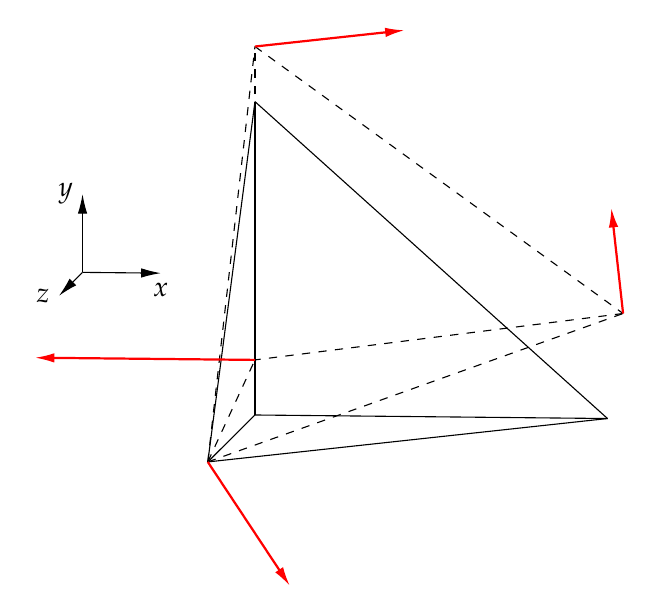
\begin{tikzpicture}
\draw[->] (-0.980017,2.03987) -- (0.0149875,2.0299);
\node[below] at (0.0149875,2.0299) {$x$};
\draw[->] (-0.980017,2.03987) -- (-0.980017,3.03487);
\node[left] at (-0.980017,3.03487) {$y$};
\draw[->] (-0.980017,2.03987) -- (-1.27952,1.74186);
\node[left] at (-1.27952,1.74186) {$z$};
\draw (1.20966,0.228594) -- (1.20966,4.20861);
\draw (1.20966,4.20861) -- (5.68718,0.183744);
\draw (5.68718,0.183744) -- (1.20966,0.228594);
\draw (0.610658,-0.367414) -- (1.20966,0.228594);
\draw (0.610658,-0.367414) -- (1.20966,4.20861);
\draw (0.610658,-0.367414) -- (5.68718,0.183744);
\draw[dashed] (1.20966,0.928164) -- (1.20966,4.90818);
\draw[dashed] (1.20966,4.90818) -- (5.88499,1.51754);
\draw[dashed] (5.88499,1.51754) -- (1.20966,0.928164);
\draw[dashed] (0.610658,-0.367414) -- (1.20966,0.928164);
\draw[dashed] (0.610658,-0.367414) -- (1.20966,4.90818);
\draw[dashed] (0.610658,-0.367414) -- (5.88499,1.51754);
\draw[->,thick,red] (5.88499,1.51754) -- (5.73524,2.86104);
\draw[->,thick,red] (1.20966,0.928164) -- (-1.58879,0.956196);
\draw[->,thick,red] (1.20966,4.90818) -- (3.11335,5.11487);
\draw[->,thick,red] (0.610658,-0.367414) -- (1.65516,-1.94563);
\end{tikzpicture}
\caption{Tetrahedron}
\label{fig:tetrahedron}
\end{figure}

\section{The Steepest Descent Method}

\begin{figure}[H]
\centering
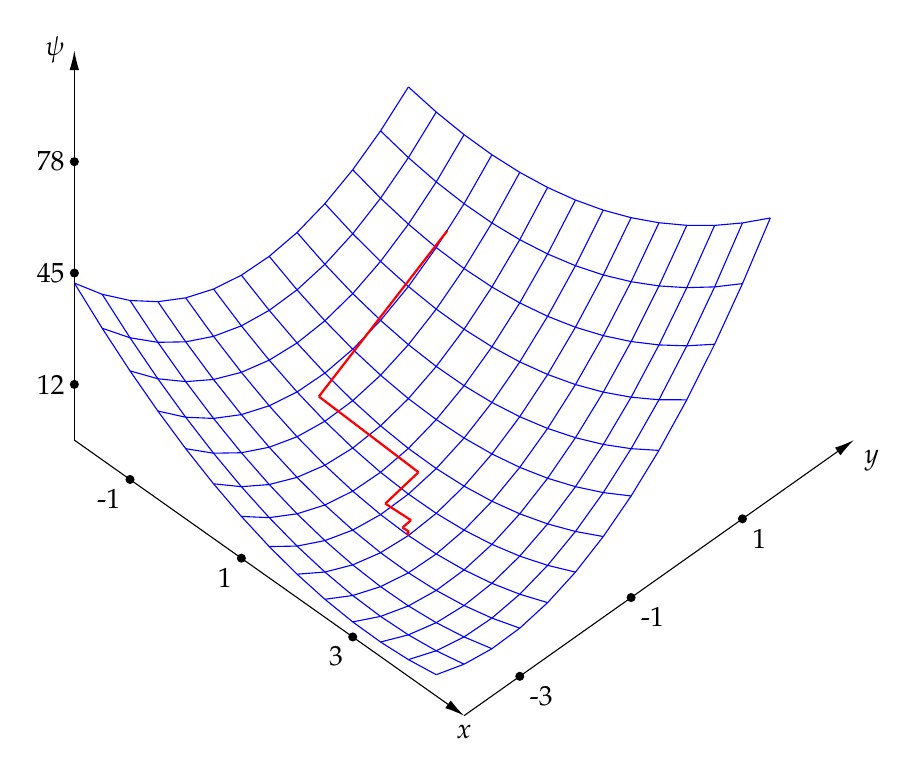
\begin{tikzpicture}
\draw[blue] (-3.88909,0.639465) -- (-4.24264,0.781909);
\draw[blue] (-3.53553,0.56066) -- (-3.88909,0.639465);
\draw[blue] (-3.18198,0.545495) -- (-3.53553,0.56066);
\draw[blue] (-2.82843,0.59397) -- (-3.18198,0.545495);
\draw[blue] (-2.47487,0.706084) -- (-2.82843,0.59397);
\draw[blue] (-2.12132,0.881838) -- (-2.47487,0.706084);
\draw[blue] (-1.76777,1.12123) -- (-2.12132,0.881838);
\draw[blue] (-1.41421,1.42426) -- (-1.76777,1.12123);
\draw[blue] (-1.06066,1.79094) -- (-1.41421,1.42426);
\draw[blue] (-0.707107,2.22125) -- (-1.06066,1.79094);
\draw[blue] (-0.353553,2.7152) -- (-0.707107,2.22125);
\draw[blue] (-2.22045e-16,3.27279) -- (-0.353553,2.7152);
\draw[blue] (-3.88909,0.208408) -- (-4.24264,0.781909);
\draw[blue] (-3.53553,0.0871767) -- (-3.88909,0.639465);
\draw[blue] (-3.53553,0.0871767) -- (-3.88909,0.208408);
\draw[blue] (-3.18198,0.0295852) -- (-3.53553,0.56066);
\draw[blue] (-3.18198,0.0295852) -- (-3.53553,0.0871767);
\draw[blue] (-2.82843,0.0356334) -- (-3.18198,0.545495);
\draw[blue] (-2.82843,0.0356334) -- (-3.18198,0.0295852);
\draw[blue] (-2.47487,0.105321) -- (-2.82843,0.59397);
\draw[blue] (-2.47487,0.105321) -- (-2.82843,0.0356334);
\draw[blue] (-2.12132,0.238649) -- (-2.47487,0.706084);
\draw[blue] (-2.12132,0.238649) -- (-2.47487,0.105321);
\draw[blue] (-1.76777,0.435616) -- (-2.12132,0.881838);
\draw[blue] (-1.76777,0.435616) -- (-2.12132,0.238649);
\draw[blue] (-1.41421,0.696222) -- (-1.76777,1.12123);
\draw[blue] (-1.41421,0.696222) -- (-1.76777,0.435616);
\draw[blue] (-1.06066,1.02047) -- (-1.41421,1.42426);
\draw[blue] (-1.06066,1.02047) -- (-1.41421,0.696222);
\draw[blue] (-0.707107,1.40835) -- (-1.06066,1.79094);
\draw[blue] (-0.707107,1.40835) -- (-1.06066,1.02047);
\draw[blue] (-0.353553,1.85988) -- (-0.707107,2.22125);
\draw[blue] (-0.353553,1.85988) -- (-0.707107,1.40835);
\draw[blue] (-1.66533e-16,2.37504) -- (-0.353553,2.7152);
\draw[blue] (-1.66533e-16,2.37504) -- (-0.353553,1.85988);
\draw[blue] (0.353553,2.95385) -- (-2.22045e-16,3.27279);
\draw[blue] (0.353553,2.95385) -- (-1.66533e-16,2.37504);
\draw[blue] (-3.53553,-0.333274) -- (-3.88909,0.208408);
\draw[blue] (-3.18198,-0.433292) -- (-3.53553,0.0871767);
\draw[blue] (-3.18198,-0.433292) -- (-3.53553,-0.333274);
\draw[blue] (-2.82843,-0.46967) -- (-3.18198,0.0295852);
\draw[blue] (-2.82843,-0.46967) -- (-3.18198,-0.433292);
\draw[blue] (-2.47487,-0.442409) -- (-2.82843,0.0356334);
\draw[blue] (-2.47487,-0.442409) -- (-2.82843,-0.46967);
\draw[blue] (-2.12132,-0.351508) -- (-2.47487,0.105321);
\draw[blue] (-2.12132,-0.351508) -- (-2.47487,-0.442409);
\draw[blue] (-1.76777,-0.196967) -- (-2.12132,0.238649);
\draw[blue] (-1.76777,-0.196967) -- (-2.12132,-0.351508);
\draw[blue] (-1.41421,0.0212132) -- (-1.76777,0.435616);
\draw[blue] (-1.41421,0.0212132) -- (-1.76777,-0.196967);
\draw[blue] (-1.06066,0.303033) -- (-1.41421,0.696222);
\draw[blue] (-1.06066,0.303033) -- (-1.41421,0.0212132);
\draw[blue] (-0.707107,0.648492) -- (-1.06066,1.02047);
\draw[blue] (-0.707107,0.648492) -- (-1.06066,0.303033);
\draw[blue] (-0.353553,1.05759) -- (-0.707107,1.40835);
\draw[blue] (-0.353553,1.05759) -- (-0.707107,0.648492);
\draw[blue] (-1.11022e-16,1.53033) -- (-0.353553,1.85988);
\draw[blue] (-1.11022e-16,1.53033) -- (-0.353553,1.05759);
\draw[blue] (0.353553,2.06671) -- (-1.66533e-16,2.37504);
\draw[blue] (0.353553,2.06671) -- (-1.11022e-16,1.53033);
\draw[blue] (0.707107,2.66673) -- (0.353553,2.95385);
\draw[blue] (0.707107,2.66673) -- (0.353553,2.06671);
\draw[blue] (-3.18198,-0.843136) -- (-3.53553,-0.333274);
\draw[blue] (-2.82843,-0.92194) -- (-3.18198,-0.433292);
\draw[blue] (-2.82843,-0.92194) -- (-3.18198,-0.843136);
\draw[blue] (-2.47487,-0.937105) -- (-2.82843,-0.46967);
\draw[blue] (-2.47487,-0.937105) -- (-2.82843,-0.92194);
\draw[blue] (-2.12132,-0.888631) -- (-2.47487,-0.442409);
\draw[blue] (-2.12132,-0.888631) -- (-2.47487,-0.937105);
\draw[blue] (-1.76777,-0.776517) -- (-2.12132,-0.351508);
\draw[blue] (-1.76777,-0.776517) -- (-2.12132,-0.888631);
\draw[blue] (-1.41421,-0.600763) -- (-1.76777,-0.196967);
\draw[blue] (-1.41421,-0.600763) -- (-1.76777,-0.776517);
\draw[blue] (-1.06066,-0.361369) -- (-1.41421,0.0212132);
\draw[blue] (-1.06066,-0.361369) -- (-1.41421,-0.600763);
\draw[blue] (-0.707107,-0.0583363) -- (-1.06066,0.303033);
\draw[blue] (-0.707107,-0.0583363) -- (-1.06066,-0.361369);
\draw[blue] (-0.353553,0.308336) -- (-0.707107,0.648492);
\draw[blue] (-0.353553,0.308336) -- (-0.707107,-0.0583363);
\draw[blue] (-5.55112e-17,0.738649) -- (-0.353553,1.05759);
\draw[blue] (-5.55112e-17,0.738649) -- (-0.353553,0.308336);
\draw[blue] (0.353553,1.2326) -- (-1.11022e-16,1.53033);
\draw[blue] (0.353553,1.2326) -- (-5.55112e-17,0.738649);
\draw[blue] (0.707107,1.79019) -- (0.353553,2.06671);
\draw[blue] (0.707107,1.79019) -- (0.353553,1.2326);
\draw[blue] (1.06066,2.41142) -- (0.707107,2.66673);
\draw[blue] (1.06066,2.41142) -- (0.707107,1.79019);
\draw[blue] (-2.82843,-1.32118) -- (-3.18198,-0.843136);
\draw[blue] (-2.47487,-1.37877) -- (-2.82843,-0.92194);
\draw[blue] (-2.47487,-1.37877) -- (-2.82843,-1.32118);
\draw[blue] (-2.12132,-1.37272) -- (-2.47487,-0.937105);
\draw[blue] (-2.12132,-1.37272) -- (-2.47487,-1.37877);
\draw[blue] (-1.76777,-1.30303) -- (-2.12132,-0.888631);
\draw[blue] (-1.76777,-1.30303) -- (-2.12132,-1.37272);
\draw[blue] (-1.41421,-1.16971) -- (-1.76777,-0.776517);
\draw[blue] (-1.41421,-1.16971) -- (-1.76777,-1.30303);
\draw[blue] (-1.06066,-0.972739) -- (-1.41421,-0.600763);
\draw[blue] (-1.06066,-0.972739) -- (-1.41421,-1.16971);
\draw[blue] (-0.707107,-0.712132) -- (-1.06066,-0.361369);
\draw[blue] (-0.707107,-0.712132) -- (-1.06066,-0.972739);
\draw[blue] (-0.353553,-0.387886) -- (-0.707107,-0.0583363);
\draw[blue] (-0.353553,-0.387886) -- (-0.707107,-0.712132);
\draw[blue] (0,0) -- (-0.353553,0.308336);
\draw[blue] (0,0) -- (-0.353553,-0.387886);
\draw[blue] (0.353553,0.451525) -- (-5.55112e-17,0.738649);
\draw[blue] (0.353553,0.451525) -- (0,0);
\draw[blue] (0.707107,0.96669) -- (0.353553,1.2326);
\draw[blue] (0.707107,0.96669) -- (0.353553,0.451525);
\draw[blue] (1.06066,1.5455) -- (0.707107,1.79019);
\draw[blue] (1.06066,1.5455) -- (0.707107,0.96669);
\draw[blue] (1.41421,2.18794) -- (1.06066,2.41142);
\draw[blue] (1.41421,2.18794) -- (1.06066,1.5455);
\draw[blue] (-2.47487,-1.7674) -- (-2.82843,-1.32118);
\draw[blue] (-2.12132,-1.80378) -- (-2.47487,-1.37877);
\draw[blue] (-2.12132,-1.80378) -- (-2.47487,-1.7674);
\draw[blue] (-1.76777,-1.77652) -- (-2.12132,-1.37272);
\draw[blue] (-1.76777,-1.77652) -- (-2.12132,-1.80378);
\draw[blue] (-1.41421,-1.68562) -- (-1.76777,-1.30303);
\draw[blue] (-1.41421,-1.68562) -- (-1.76777,-1.77652);
\draw[blue] (-1.06066,-1.53107) -- (-1.41421,-1.16971);
\draw[blue] (-1.06066,-1.53107) -- (-1.41421,-1.68562);
\draw[blue] (-0.707107,-1.31289) -- (-1.06066,-0.972739);
\draw[blue] (-0.707107,-1.31289) -- (-1.06066,-1.53107);
\draw[blue] (-0.353553,-1.03107) -- (-0.707107,-0.712132);
\draw[blue] (-0.353553,-1.03107) -- (-0.707107,-1.31289);
\draw[blue] (5.55112e-17,-0.685616) -- (-0.353553,-0.387886);
\draw[blue] (5.55112e-17,-0.685616) -- (-0.353553,-1.03107);
\draw[blue] (0.353553,-0.276517) -- (0,0);
\draw[blue] (0.353553,-0.276517) -- (5.55112e-17,-0.685616);
\draw[blue] (0.707107,0.196222) -- (0.353553,0.451525);
\draw[blue] (0.707107,0.196222) -- (0.353553,-0.276517);
\draw[blue] (1.06066,0.7326) -- (0.707107,0.96669);
\draw[blue] (1.06066,0.7326) -- (0.707107,0.196222);
\draw[blue] (1.41421,1.33262) -- (1.06066,1.5455);
\draw[blue] (1.41421,1.33262) -- (1.06066,0.7326);
\draw[blue] (1.76777,1.99628) -- (1.41421,2.18794);
\draw[blue] (1.76777,1.99628) -- (1.41421,1.33262);
\draw[blue] (-2.12132,-2.1818) -- (-2.47487,-1.7674);
\draw[blue] (-1.76777,-2.19697) -- (-2.12132,-1.80378);
\draw[blue] (-1.76777,-2.19697) -- (-2.12132,-2.1818);
\draw[blue] (-1.41421,-2.14849) -- (-1.76777,-1.77652);
\draw[blue] (-1.41421,-2.14849) -- (-1.76777,-2.19697);
\draw[blue] (-1.06066,-2.03638) -- (-1.41421,-1.68562);
\draw[blue] (-1.06066,-2.03638) -- (-1.41421,-2.14849);
\draw[blue] (-0.707107,-1.86062) -- (-1.06066,-1.53107);
\draw[blue] (-0.707107,-1.86062) -- (-1.06066,-2.03638);
\draw[blue] (-0.353553,-1.62123) -- (-0.707107,-1.31289);
\draw[blue] (-0.353553,-1.62123) -- (-0.707107,-1.86062);
\draw[blue] (1.11022e-16,-1.3182) -- (-0.353553,-1.03107);
\draw[blue] (1.11022e-16,-1.3182) -- (-0.353553,-1.62123);
\draw[blue] (0.353553,-0.951525) -- (5.55112e-17,-0.685616);
\draw[blue] (0.353553,-0.951525) -- (1.11022e-16,-1.3182);
\draw[blue] (0.707107,-0.521213) -- (0.353553,-0.276517);
\draw[blue] (0.707107,-0.521213) -- (0.353553,-0.951525);
\draw[blue] (1.06066,-0.0272614) -- (0.707107,0.196222);
\draw[blue] (1.06066,-0.0272614) -- (0.707107,-0.521213);
\draw[blue] (1.41421,0.53033) -- (1.06066,0.7326);
\draw[blue] (1.41421,0.53033) -- (1.06066,-0.0272614);
\draw[blue] (1.76777,1.15156) -- (1.41421,1.33262);
\draw[blue] (1.76777,1.15156) -- (1.41421,0.53033);
\draw[blue] (2.12132,1.83643) -- (1.76777,1.99628);
\draw[blue] (2.12132,1.83643) -- (1.76777,1.15156);
\draw[blue] (-1.76777,-2.56438) -- (-2.12132,-2.1818);
\draw[blue] (-1.41421,-2.55834) -- (-1.76777,-2.19697);
\draw[blue] (-1.41421,-2.55834) -- (-1.76777,-2.56438);
\draw[blue] (-1.06066,-2.48865) -- (-1.41421,-2.14849);
\draw[blue] (-1.06066,-2.48865) -- (-1.41421,-2.55834);
\draw[blue] (-0.707107,-2.35532) -- (-1.06066,-2.03638);
\draw[blue] (-0.707107,-2.35532) -- (-1.06066,-2.48865);
\draw[blue] (-0.353553,-2.15835) -- (-0.707107,-1.86062);
\draw[blue] (-0.353553,-2.15835) -- (-0.707107,-2.35532);
\draw[blue] (1.66533e-16,-1.89775) -- (-0.353553,-1.62123);
\draw[blue] (1.66533e-16,-1.89775) -- (-0.353553,-2.15835);
\draw[blue] (0.353553,-1.5735) -- (1.11022e-16,-1.3182);
\draw[blue] (0.353553,-1.5735) -- (1.66533e-16,-1.89775);
\draw[blue] (0.707107,-1.18562) -- (0.353553,-0.951525);
\draw[blue] (0.707107,-1.18562) -- (0.353553,-1.5735);
\draw[blue] (1.06066,-0.73409) -- (0.707107,-0.521213);
\draw[blue] (1.06066,-0.73409) -- (0.707107,-1.18562);
\draw[blue] (1.41421,-0.218925) -- (1.06066,-0.0272614);
\draw[blue] (1.41421,-0.218925) -- (1.06066,-0.73409);
\draw[blue] (1.76777,0.35988) -- (1.41421,0.53033);
\draw[blue] (1.76777,0.35988) -- (1.41421,-0.218925);
\draw[blue] (2.12132,1.00232) -- (1.76777,1.15156);
\draw[blue] (2.12132,1.00232) -- (1.76777,0.35988);
\draw[blue] (2.47487,1.70841) -- (2.12132,1.83643);
\draw[blue] (2.47487,1.70841) -- (2.12132,1.00232);
\draw[blue] (-1.41421,-2.91515) -- (-1.76777,-2.56438);
\draw[blue] (-1.06066,-2.88789) -- (-1.41421,-2.55834);
\draw[blue] (-1.06066,-2.88789) -- (-1.41421,-2.91515);
\draw[blue] (-0.707107,-2.79698) -- (-1.06066,-2.48865);
\draw[blue] (-0.707107,-2.79698) -- (-1.06066,-2.88789);
\draw[blue] (-0.353553,-2.64244) -- (-0.707107,-2.35532);
\draw[blue] (-0.353553,-2.64244) -- (-0.707107,-2.79698);
\draw[blue] (2.22045e-16,-2.42426) -- (-0.353553,-2.15835);
\draw[blue] (2.22045e-16,-2.42426) -- (-0.353553,-2.64244);
\draw[blue] (0.353553,-2.14244) -- (1.66533e-16,-1.89775);
\draw[blue] (0.353553,-2.14244) -- (2.22045e-16,-2.42426);
\draw[blue] (0.707107,-1.79698) -- (0.353553,-1.5735);
\draw[blue] (0.707107,-1.79698) -- (0.353553,-2.14244);
\draw[blue] (1.06066,-1.38789) -- (0.707107,-1.18562);
\draw[blue] (1.06066,-1.38789) -- (0.707107,-1.79698);
\draw[blue] (1.41421,-0.915147) -- (1.06066,-0.73409);
\draw[blue] (1.41421,-0.915147) -- (1.06066,-1.38789);
\draw[blue] (1.76777,-0.378769) -- (1.41421,-0.218925);
\draw[blue] (1.76777,-0.378769) -- (1.41421,-0.915147);
\draw[blue] (2.12132,0.221249) -- (1.76777,0.35988);
\draw[blue] (2.12132,0.221249) -- (1.76777,-0.378769);
\draw[blue] (2.47487,0.884906) -- (2.12132,1.00232);
\draw[blue] (2.47487,0.884906) -- (2.12132,0.221249);
\draw[blue] (2.82843,1.6122) -- (2.47487,1.70841);
\draw[blue] (2.82843,1.6122) -- (2.47487,0.884906);
\draw[blue] (-1.06066,-3.23409) -- (-1.41421,-2.91515);
\draw[blue] (-0.707107,-3.18562) -- (-1.06066,-2.88789);
\draw[blue] (-0.707107,-3.18562) -- (-1.06066,-3.23409);
\draw[blue] (-0.353553,-3.0735) -- (-0.707107,-2.79698);
\draw[blue] (-0.353553,-3.0735) -- (-0.707107,-3.18562);
\draw[blue] (2.77556e-16,-2.89775) -- (-0.353553,-2.64244);
\draw[blue] (2.77556e-16,-2.89775) -- (-0.353553,-3.0735);
\draw[blue] (0.353553,-2.65835) -- (2.22045e-16,-2.42426);
\draw[blue] (0.353553,-2.65835) -- (2.77556e-16,-2.89775);
\draw[blue] (0.707107,-2.35532) -- (0.353553,-2.14244);
\draw[blue] (0.707107,-2.35532) -- (0.353553,-2.65835);
\draw[blue] (1.06066,-1.98865) -- (0.707107,-1.79698);
\draw[blue] (1.06066,-1.98865) -- (0.707107,-2.35532);
\draw[blue] (1.41421,-1.55834) -- (1.06066,-1.38789);
\draw[blue] (1.41421,-1.55834) -- (1.06066,-1.98865);
\draw[blue] (1.76777,-1.06438) -- (1.41421,-0.915147);
\draw[blue] (1.76777,-1.06438) -- (1.41421,-1.55834);
\draw[blue] (2.12132,-0.506793) -- (1.76777,-0.378769);
\draw[blue] (2.12132,-0.506793) -- (1.76777,-1.06438);
\draw[blue] (2.47487,0.114438) -- (2.12132,0.221249);
\draw[blue] (2.47487,0.114438) -- (2.12132,-0.506793);
\draw[blue] (2.82843,0.799309) -- (2.47487,0.884906);
\draw[blue] (2.82843,0.799309) -- (2.47487,0.114438);
\draw[blue] (3.18198,1.54782) -- (2.82843,1.6122);
\draw[blue] (3.18198,1.54782) -- (2.82843,0.799309);
\draw[blue] (-0.707107,-3.52121) -- (-1.06066,-3.23409);
\draw[blue] (-0.353553,-3.45153) -- (-0.707107,-3.18562);
\draw[blue] (-0.353553,-3.45153) -- (-0.707107,-3.52121);
\draw[blue] (3.33067e-16,-3.3182) -- (-0.353553,-3.0735);
\draw[blue] (3.33067e-16,-3.3182) -- (-0.353553,-3.45153);
\draw[blue] (0.353553,-3.12123) -- (2.77556e-16,-2.89775);
\draw[blue] (0.353553,-3.12123) -- (3.33067e-16,-3.3182);
\draw[blue] (0.707107,-2.86062) -- (0.353553,-2.65835);
\draw[blue] (0.707107,-2.86062) -- (0.353553,-3.12123);
\draw[blue] (1.06066,-2.53638) -- (0.707107,-2.35532);
\draw[blue] (1.06066,-2.53638) -- (0.707107,-2.86062);
\draw[blue] (1.41421,-2.14849) -- (1.06066,-1.98865);
\draw[blue] (1.41421,-2.14849) -- (1.06066,-2.53638);
\draw[blue] (1.76777,-1.69697) -- (1.41421,-1.55834);
\draw[blue] (1.76777,-1.69697) -- (1.41421,-2.14849);
\draw[blue] (2.12132,-1.1818) -- (1.76777,-1.06438);
\draw[blue] (2.12132,-1.1818) -- (1.76777,-1.69697);
\draw[blue] (2.47487,-0.602997) -- (2.12132,-0.506793);
\draw[blue] (2.47487,-0.602997) -- (2.12132,-1.1818);
\draw[blue] (2.82843,0.039447) -- (2.47487,0.114438);
\draw[blue] (2.82843,0.039447) -- (2.47487,-0.602997);
\draw[blue] (3.18198,0.745531) -- (2.82843,0.799309);
\draw[blue] (3.18198,0.745531) -- (2.82843,0.039447);
\draw[blue] (3.53553,1.51525) -- (3.18198,1.54782);
\draw[blue] (3.53553,1.51525) -- (3.18198,0.745531);
\draw[blue] (-0.353553,-3.77652) -- (-0.707107,-3.52121);
\draw[blue] (3.88578e-16,-3.68562) -- (-0.353553,-3.45153);
\draw[blue] (3.88578e-16,-3.68562) -- (-0.353553,-3.77652);
\draw[blue] (0.353553,-3.53107) -- (3.33067e-16,-3.3182);
\draw[blue] (0.353553,-3.53107) -- (3.88578e-16,-3.68562);
\draw[blue] (0.707107,-3.31289) -- (0.353553,-3.12123);
\draw[blue] (0.707107,-3.31289) -- (0.353553,-3.53107);
\draw[blue] (1.06066,-3.03107) -- (0.707107,-2.86062);
\draw[blue] (1.06066,-3.03107) -- (0.707107,-3.31289);
\draw[blue] (1.41421,-2.68562) -- (1.06066,-2.53638);
\draw[blue] (1.41421,-2.68562) -- (1.06066,-3.03107);
\draw[blue] (1.76777,-2.27652) -- (1.41421,-2.14849);
\draw[blue] (1.76777,-2.27652) -- (1.41421,-2.68562);
\draw[blue] (2.12132,-1.80378) -- (1.76777,-1.69697);
\draw[blue] (2.12132,-1.80378) -- (1.76777,-2.27652);
\draw[blue] (2.47487,-1.2674) -- (2.12132,-1.1818);
\draw[blue] (2.47487,-1.2674) -- (2.12132,-1.80378);
\draw[blue] (2.82843,-0.667382) -- (2.47487,-0.602997);
\draw[blue] (2.82843,-0.667382) -- (2.47487,-1.2674);
\draw[blue] (3.18198,-0.0037243) -- (2.82843,0.039447);
\draw[blue] (3.18198,-0.0037243) -- (2.82843,-0.667382);
\draw[blue] (3.53553,0.723573) -- (3.18198,0.745531);
\draw[blue] (3.53553,0.723573) -- (3.18198,-0.0037243);
\draw[blue] (3.88909,1.51451) -- (3.53553,1.51525);
\draw[blue] (3.88909,1.51451) -- (3.53553,0.723573);
\draw[blue] (4.44089e-16,-4) -- (-0.353553,-3.77652);
\draw[blue] (0.353553,-3.88789) -- (3.88578e-16,-3.68562);
\draw[blue] (0.353553,-3.88789) -- (4.44089e-16,-4);
\draw[blue] (0.707107,-3.71213) -- (0.353553,-3.53107);
\draw[blue] (0.707107,-3.71213) -- (0.353553,-3.88789);
\draw[blue] (1.06066,-3.47274) -- (0.707107,-3.31289);
\draw[blue] (1.06066,-3.47274) -- (0.707107,-3.71213);
\draw[blue] (1.41421,-3.16971) -- (1.06066,-3.03107);
\draw[blue] (1.41421,-3.16971) -- (1.06066,-3.47274);
\draw[blue] (1.76777,-2.80303) -- (1.41421,-2.68562);
\draw[blue] (1.76777,-2.80303) -- (1.41421,-3.16971);
\draw[blue] (2.12132,-2.37272) -- (1.76777,-2.27652);
\draw[blue] (2.12132,-2.37272) -- (1.76777,-2.80303);
\draw[blue] (2.47487,-1.87877) -- (2.12132,-1.80378);
\draw[blue] (2.47487,-1.87877) -- (2.12132,-2.37272);
\draw[blue] (2.82843,-1.32118) -- (2.47487,-1.2674);
\draw[blue] (2.82843,-1.32118) -- (2.47487,-1.87877);
\draw[blue] (3.18198,-0.699946) -- (2.82843,-0.667382);
\draw[blue] (3.18198,-0.699946) -- (2.82843,-1.32118);
\draw[blue] (3.53553,-0.0150758) -- (3.18198,-0.0037243);
\draw[blue] (3.53553,-0.0150758) -- (3.18198,-0.699946);
\draw[blue] (3.88909,0.733435) -- (3.53553,0.723573);
\draw[blue] (3.88909,0.733435) -- (3.53553,-0.0150758);
\draw[blue] (4.24264,1.54558) -- (3.88909,1.51451);
\draw[blue] (4.24264,1.54558) -- (3.88909,0.733435);
\draw[blue] (0.353553,-4.19166) -- (4.44089e-16,-4);
\draw[blue] (0.707107,-4.05834) -- (0.353553,-3.88789);
\draw[blue] (0.707107,-4.05834) -- (0.353553,-4.19166);
\draw[blue] (1.06066,-3.86137) -- (0.707107,-3.71213);
\draw[blue] (1.06066,-3.86137) -- (0.707107,-4.05834);
\draw[blue] (1.41421,-3.60076) -- (1.06066,-3.47274);
\draw[blue] (1.41421,-3.60076) -- (1.06066,-3.86137);
\draw[blue] (1.76777,-3.27652) -- (1.41421,-3.16971);
\draw[blue] (1.76777,-3.27652) -- (1.41421,-3.60076);
\draw[blue] (2.12132,-2.88863) -- (1.76777,-2.80303);
\draw[blue] (2.12132,-2.88863) -- (1.76777,-3.27652);
\draw[blue] (2.47487,-2.43711) -- (2.12132,-2.37272);
\draw[blue] (2.47487,-2.43711) -- (2.12132,-2.88863);
\draw[blue] (2.82843,-1.92194) -- (2.47487,-1.87877);
\draw[blue] (2.82843,-1.92194) -- (2.47487,-2.43711);
\draw[blue] (3.18198,-1.34314) -- (2.82843,-1.32118);
\draw[blue] (3.18198,-1.34314) -- (2.82843,-1.92194);
\draw[blue] (3.53553,-0.700691) -- (3.18198,-0.699946);
\draw[blue] (3.53553,-0.700691) -- (3.18198,-1.34314);
\draw[blue] (3.88909,0.00539258) -- (3.53553,-0.0150758);
\draw[blue] (3.88909,0.00539258) -- (3.53553,-0.700691);
\draw[blue] (4.24264,0.775116) -- (3.88909,0.733435);
\draw[blue] (4.24264,0.775116) -- (3.88909,0.00539258);
\draw[blue] (4.59619,1.60848) -- (4.24264,1.54558);
\draw[blue] (4.59619,1.60848) -- (4.24264,0.775116);
\draw[->] (-4.24264,-1.21213) -- (0.707107,-4.71213);
\draw[->] (0.707107,-4.71213) -- (5.65685,-1.21213);
\draw[->] (-4.24264,-1.21213) -- (-4.24264,3.73762);
\node[below] at (0.707107,-4.71213) {$x$};
\node[below right] at (5.65685,-1.21213) {$y$};
\node[left] at (-4.24264,3.73762) {$\psi$};
\draw[fill] (-3.53553,-1.71213) circle(0.05);
\node[below left] at (-3.53553,-1.71213) {-1};
\draw[fill] (1.41421,-4.21213) circle(0.05);
\node[below right] at (1.41421,-4.21213) {-3};
\draw[fill] (-4.24264,-0.505025) circle(0.05);
\node[left] at (-4.24264,-0.505025) {12};
\draw[fill] (-2.12132,-2.71213) circle(0.05);
\node[below left] at (-2.12132,-2.71213) {1};
\draw[fill] (2.82843,-3.21213) circle(0.05);
\node[below right] at (2.82843,-3.21213) {-1};
\draw[fill] (-4.24264,0.909188) circle(0.05);
\node[left] at (-4.24264,0.909188) {45};
\draw[fill] (-0.707107,-3.71213) circle(0.05);
\node[below left] at (-0.707107,-3.71213) {3};
\draw[fill] (4.24264,-2.21213) circle(0.05);
\node[below right] at (4.24264,-2.21213) {1};
\draw[fill] (-4.24264,2.3234) circle(0.05);
\node[left] at (-4.24264,2.3234) {78};
\draw[thick,red] (0.494975,1.448) -- (-1.13755,-0.658609);
\draw[thick,red] (-1.13755,-0.658609) -- (0.127773,-1.62044);
\draw[thick,red] (0.127773,-1.62044) -- (-0.293648,-2.01901);
\draw[thick,red] (-0.293648,-2.01901) -- (0.0329834,-2.22981);
\draw[thick,red] (0.0329834,-2.22981) -- (-0.0758025,-2.32302);
\draw[thick,red] (-0.0758025,-2.32302) -- (0.00851437,-2.37494);
\draw[thick,red] (0.00851437,-2.37494) -- (-0.0195677,-2.39835);
\draw[thick,red] (-0.0195677,-2.39835) -- (0.00219791,-2.41159);
\draw[thick,red] (0.00219791,-2.41159) -- (-0.00505122,-2.41759);
\draw[thick,red] (-0.00505122,-2.41759) -- (0.000567369,-2.421);
\end{tikzpicture}
\caption{Quadratic Form}
\label{fig:quadratic-form}
\end{figure}

\begin{figure}[H]
\centering
\begin{tikzpicture}
\draw[<->] (-4,0) -- (8,0);
\draw[<->] (0,-6) -- (0,2);
\draw plot[smooth cycle] coordinates {(-1.07838,1.11093) (-1.64236,0.908924) (-2.16072,0.52681) (-2.43369,0.100035) (-2.54387,-0.436686) (-2.47123,-1.01657) (-2.25492,-1.57723) (-1.94222,-2.09586) (-1.56414,-2.57024) (-1.13875,-3.00325) (-0.713718,-3.3687) (-0.260188,-3.70527) (0.217106,-4.01252) (0.7147,-4.28988) (1.22997,-4.53637) (1.76085,-4.75038) (2.30559,-4.92947) (2.86255,-5.07002) (3.42996,-5.16672) (4.00548,-5.21164) (4.58538,-5.19251) (5.16273,-5.08935) (5.72264,-4.86643) (6.22938,-4.44678) (6.47252,-3.9934) (6.54301,-3.44084) (6.43544,-2.86122) (6.19515,-2.30866) (5.86648,-1.79957) (5.47714,-1.33428) (5.04323,-0.90964) (4.6111,-0.550822) (4.1517,-0.221002) (3.66944,0.079392) (3.16755,0.349713) (2.64849,0.588853) (2.11426,0.795037) (1.56655,0.965584) (1.007,1.09654) (0.437471,1.18208) (-0.13947,1.21348) (-0.719583,1.17708)};
\draw[thick,red] (-0.5,1.2) -- (-0.306136,-1.3026);
\draw plot[smooth cycle] coordinates {(-0.223974,-1.64576) (-0.0582406,-1.96648) (0.159735,-2.25623) (0.412658,-2.51656) (0.66549,-2.7302) (0.937538,-2.92425) (1.22525,-3.09817) (1.52614,-3.25129) (1.83834,-3.38247) (2.16038,-3.48988) (2.49095,-3.57062) (2.8286,-3.62019) (3.17129,-3.63131) (3.51528,-3.59155) (3.85218,-3.47716) (4.15947,-3.22951) (4.28816,-2.9556) (4.29719,-2.62044) (4.19295,-2.28028) (4.01345,-1.96634) (3.78657,-1.68336) (3.5273,-1.42921) (3.26935,-1.22033) (2.99317,-1.03117) (2.70202,-0.862279) (2.39821,-0.714416) (2.08347,-0.588868) (1.75921,-0.487691) (1.42675,-0.414104) (1.08764,-0.37316) (0.744181,-0.373093) (0.400859,-0.428294) (0.0681931,-0.567386) (-0.224431,-0.872464) (-0.307371,-1.17729) (-0.266092,-1.52084)};
\draw[thick,red] (-0.306136,-1.3026) -- (1.35465,-1.17395);
\draw plot[smooth cycle] coordinates {(1.20534,-1.19694) (1.05976,-1.24909) (0.925949,-1.34773) (0.855485,-1.4579) (0.827042,-1.59645) (0.845793,-1.74614) (0.901632,-1.89087) (0.982353,-2.02475) (1.07995,-2.1472) (1.18976,-2.25898) (1.29948,-2.35332) (1.41655,-2.4402) (1.53976,-2.51951) (1.66821,-2.59111) (1.80122,-2.65474) (1.93827,-2.70998) (2.07888,-2.75621) (2.22266,-2.7925) (2.36913,-2.81746) (2.5177,-2.82905) (2.66739,-2.82412) (2.81643,-2.79749) (2.96096,-2.73994) (3.09178,-2.63161) (3.15454,-2.51458) (3.17274,-2.37194) (3.14497,-2.22232) (3.08294,-2.07968) (2.9981,-1.94826) (2.89759,-1.82815) (2.78558,-1.71853) (2.67403,-1.62591) (2.55544,-1.54077) (2.43095,-1.46322) (2.30139,-1.39344) (2.1674,-1.33171) (2.0295,-1.27849) (1.88811,-1.23446) (1.74367,-1.20066) (1.59665,-1.17857) (1.44772,-1.17047) (1.29797,-1.17987)};
\draw[thick,red] (1.35465,-1.17395) -- (1.40469,-1.81997);
\draw plot[smooth cycle] coordinates {(1.4259,-1.90856) (1.46868,-1.99135) (1.52495,-2.06614) (1.59024,-2.13335) (1.65551,-2.1885) (1.72574,-2.23859) (1.80001,-2.28348) (1.87768,-2.32301) (1.95827,-2.35687) (2.0414,-2.3846) (2.12673,-2.40544) (2.2139,-2.41824) (2.30236,-2.42111) (2.39115,-2.41084) (2.47812,-2.38131) (2.55745,-2.31739) (2.59067,-2.24668) (2.593,-2.16016) (2.56609,-2.07235) (2.51975,-1.99131) (2.46119,-1.91826) (2.39426,-1.85266) (2.32767,-1.79873) (2.25638,-1.74991) (2.18122,-1.70631) (2.10279,-1.66814) (2.02155,-1.63573) (1.93784,-1.60961) (1.85202,-1.59062) (1.76448,-1.58005) (1.67582,-1.58003) (1.5872,-1.59428) (1.50132,-1.63018) (1.42578,-1.70894) (1.40437,-1.78763) (1.41503,-1.87631)};
\draw[thick,red] (1.40469,-1.81997) -- (1.83341,-1.78676);
\draw plot[smooth cycle] coordinates {(1.79487,-1.7927) (1.75729,-1.80616) (1.72274,-1.83162) (1.70455,-1.86006) (1.69721,-1.89583) (1.70205,-1.93447) (1.71647,-1.97183) (1.7373,-2.00639) (1.7625,-2.038) (1.79084,-2.06685) (1.81917,-2.09121) (1.84939,-2.11363) (1.88119,-2.13411) (1.91435,-2.15259) (1.94869,-2.16901) (1.98406,-2.18328) (2.02036,-2.19521) (2.05748,-2.20458) (2.09529,-2.21102) (2.13364,-2.21401) (2.17228,-2.21274) (2.21075,-2.20586) (2.24806,-2.19101) (2.28183,-2.16305) (2.29803,-2.13283) (2.30273,-2.09601) (2.29556,-2.05739) (2.27955,-2.02057) (2.25765,-1.98664) (2.23171,-1.95564) (2.20279,-1.92734) (2.17399,-1.90343) (2.14338,-1.88145) (2.11125,-1.86144) (2.0778,-1.84342) (2.04321,-1.82749) (2.00761,-1.81375) (1.97112,-1.80238) (1.93383,-1.79366) (1.89588,-1.78796) (1.85743,-1.78586) (1.81878,-1.78829)};
\draw[thick,red] (1.83341,-1.78676) -- (1.84633,-1.95353);
\draw plot[smooth cycle] coordinates {(1.8518,-1.97639) (1.86285,-1.99777) (1.87737,-2.01707) (1.89422,-2.03442) (1.91107,-2.04866) (1.9292,-2.06159) (1.94837,-2.07318) (1.96842,-2.08338) (1.98923,-2.09212) (2.01069,-2.09928) (2.03272,-2.10466) (2.05522,-2.10796) (2.07805,-2.1087) (2.10097,-2.10606) (2.12342,-2.09843) (2.1439,-2.08193) (2.15248,-2.06368) (2.15308,-2.04134) (2.14613,-2.01868) (2.13417,-1.99776) (2.11905,-1.9789) (2.10177,-1.96196) (2.08459,-1.94805) (2.06618,-1.93544) (2.04678,-1.92419) (2.02654,-1.91433) (2.00556,-1.90597) (1.98395,-1.89922) (1.9618,-1.89432) (1.9392,-1.89159) (1.91632,-1.89159) (1.89344,-1.89527) (1.87127,-1.90454) (1.85177,-1.92486) (1.84624,-1.94518) (1.849,-1.96807)};
\draw[thick,red] (1.84633,-1.95353) -- (1.957,-1.94495);
\draw plot[smooth cycle] coordinates {(1.94705,-1.94649) (1.93735,-1.94996) (1.92843,-1.95653) (1.92373,-1.96388) (1.92184,-1.97311) (1.92309,-1.98308) (1.92681,-1.99273) (1.93219,-2.00165) (1.93869,-2.00981) (1.94601,-2.01726) (1.95332,-2.02354) (1.96112,-2.02933) (1.96933,-2.03462) (1.97789,-2.03939) (1.98675,-2.04363) (1.99589,-2.04731) (2.00526,-2.05039) (2.01484,-2.05281) (2.0246,-2.05447) (2.0345,-2.05525) (2.04447,-2.05492) (2.0544,-2.05314) (2.06404,-2.04931) (2.07275,-2.04209) (2.07693,-2.03429) (2.07815,-2.02478) (2.0763,-2.01481) (2.07216,-2.00531) (2.06651,-1.99655) (2.05981,-1.98855) (2.05235,-1.98124) (2.04492,-1.97507) (2.03701,-1.9694) (2.02872,-1.96423) (2.02008,-1.95958) (2.01116,-1.95547) (2.00197,-1.95192) (1.99254,-1.94899) (1.98292,-1.94673) (1.97312,-1.94526) (1.9632,-1.94472) (1.95322,-1.94535)};
\draw[thick,red] (1.957,-1.94495) -- (1.96033,-1.988);
\draw plot[smooth cycle] coordinates {(1.96174,-1.99391) (1.96459,-1.99942) (1.96834,-2.00441) (1.9727,-2.00889) (1.97704,-2.01256) (1.98172,-2.0159) (1.98667,-2.01889) (1.99185,-2.02152) (1.99722,-2.02378) (2.00276,-2.02563) (2.00845,-2.02702) (2.01425,-2.02787) (2.02015,-2.02806) (2.02607,-2.02738) (2.03186,-2.02541) (2.03715,-2.02115) (2.03936,-2.01644) (2.03952,-2.01067) (2.03772,-2.00482) (2.03463,-1.99942) (2.03073,-1.99455) (2.02627,-1.99018) (2.02183,-1.98659) (2.01708,-1.98333) (2.01208,-1.98043) (2.00685,-1.97789) (2.00144,-1.97573) (1.99586,-1.97399) (1.99014,-1.97272) (1.98431,-1.97202) (1.9784,-1.97201) (1.97249,-1.97296) (1.96677,-1.97536) (1.96174,-1.9806) (1.96031,-1.98585) (1.96102,-1.99176)};
\draw[thick,red] (1.96033,-1.988) -- (1.9889,-1.98579);
\draw plot[smooth cycle] coordinates {(1.98633,-1.98619) (1.98383,-1.98708) (1.98152,-1.98878) (1.98031,-1.99067) (1.97982,-1.99306) (1.98015,-1.99563) (1.98111,-1.99812) (1.98249,-2.00043) (1.98417,-2.00253) (1.98606,-2.00445) (1.98795,-2.00608) (1.98996,-2.00757) (1.99208,-2.00894) (1.99429,-2.01017) (1.99658,-2.01126) (1.99894,-2.01221) (2.00136,-2.01301) (2.00383,-2.01363) (2.00635,-2.01406) (2.00891,-2.01426) (2.01148,-2.01418) (2.01404,-2.01372) (2.01653,-2.01273) (2.01878,-2.01086) (2.01986,-2.00885) (2.02017,-2.0064) (2.0197,-2.00382) (2.01863,-2.00137) (2.01717,-1.99911) (2.01544,-1.99704) (2.01351,-1.99516) (2.01159,-1.99357) (2.00955,-1.9921) (2.00741,-1.99077) (2.00518,-1.98957) (2.00288,-1.9885) (2.00051,-1.98759) (1.99808,-1.98683) (1.99559,-1.98625) (1.99306,-1.98587) (1.9905,-1.98573) (1.98792,-1.98589)};
\draw[thick,red] (1.9889,-1.98579) -- (1.98976,-1.9969);
\end{tikzpicture}
\caption{Intersection for $\psi = 0$}
\label{fig:levels}
\end{figure}

\section{Conjugate Gradients Method}

\begin{eqnarray}
A x = f \\
\Phi = \frac 1 2 x^T A x + x^T f \\
\nabla \Phi = \frac 1 2 I A x + \frac 1 2 x^T A I - I f \\
\nabla \Phi =
\begin{bmatrix}
\frac{\partial \Phi}{\partial x_1} \\
\frac{\partial \Phi}{\partial x_2} \\
\vdots \\
\frac{\partial \Phi}{\partial x_n}
\end{bmatrix} \\
\nabla \Phi = A x - f \\
x = x_0 + P s \\
p_i^T A p_j = 0\;\;\mbox{for}\;\;i \neq j \\
P^T A P = D \\
d_i = p_i^T A p_i \\
\nabla \Phi = A x - f = A x_0 + A P s - f \\
\nabla \Phi = A P s + r_0 \\
r_0 = f - A x_0 \\
P^T A P s + P^T r_0 = 0 \\
D s + P^T r_0 = 0 \\
s_i = \frac{p_i^T r_0}{p_i^T A p_i} \\
x = x_0 + P s
\end{eqnarray}

\section{Calculations for Tetrahedron}

\begin{figure}[H]
\centering
\begin{equation}
\begin{bmatrix}
250 & -250 & . & . & . \\
-250 & 366 & 82.47 & -73.31 & . \\
. & 82.47 & 363 & -82.47 & -64 \\
. & -73.31 & -82.47 & 73.31 & . \\
. & . & -64 & . & 85.33
\end{bmatrix}
\begin{bmatrix}
0.7031 \\
0.7031 \\
0.2531 \\
1.397 \\
0.5414
\end{bmatrix}=
\begin{bmatrix}
. \\
. \\
. \\
30 \\
30
\end{bmatrix}
\end{equation}
\caption{Equation K for Tetrahedron}
\label{eq:K}
\end{figure}

\begin{figure}[H]
\centering
\begin{equation}
\begin{bmatrix}
. & 64 & 64 & . & -85.33 \\
. & -42.67 & . & . & . \\
. & . & -48 & . & 64 \\
. & -64 & . & . & . \\
. & -82.47 & -92.78 & 82.47 & . \\
. & . & . & . & . \\
. & . & -222.2 & . & .
\end{bmatrix}
\begin{bmatrix}
0.7031 \\
0.7031 \\
0.2531 \\
1.397 \\
0.5414
\end{bmatrix}=
\begin{bmatrix}
15 \\
-30 \\
22.5 \\
-45 \\
33.75 \\
. \\
-56.25
\end{bmatrix}
\end{equation}
\caption{Equation T for Tetrahedron}
\label{eq:T}
\end{figure}

\end{document}
